\documentclass[
	12pt,				% tamanho da fonte
	oneside,			% para impressão em verso e anverso. Oposto a oneside
	a4paper,			% tamanho do papel. 
	brazil				% o último idioma é o principal do documento]{article}
]{abntex2}

% ---
% Pacotes básicos 
% ---
\usepackage{fontspec}

\usepackage[utf8]{inputenc}		% Codificacao do documento (conversão automática dos acentos)
\usepackage[T1]{fontenc}
\usepackage{indentfirst}		% Indenta o primeiro parágrafo de cada seção.
\usepackage{color}				% Controle das cores
\usepackage{graphicx}			% Inclusão de gráficos
\usepackage{microtype} 			% para melhorias de justificação
\usepackage{multicol}			% multiplas colunas no texto 
\usepackage{booktabs}

% ---

% ---
% Pacotes de citações
% ---
\usepackage[brazilian]{backref}	 % Paginas com as citações na bibl
\usepackage[alf]{abntex2cite}	% Citações padrão ABNT


\usepackage{hyperref} % criar hyperlinks
\usepackage{listings} % utilizado para dar highlight em código
\usepackage[dvipsnames]{xcolor}
\usepackage[export]{adjustbox}

% --- 
\usepackage{hyperref} % criar hyperlinks
\usepackage{listings} % utilizado para dar highlight em código
\usepackage[dvipsnames]{xcolor}
\usepackage[export]{adjustbox}
\usepackage[top=3cm, bottom=2cm, left=3cm, right=2cm]{geometry}
\renewcommand{\baselinestretch}{1.5} % espaçamento entre linhas
%\setlength{\parskip}{0.5cm} % espaçamento entre paragrafos
%\setlength{\parindent}{2cm} % recuo do parágrafo
\usepackage{times}
% ---


\lstdefinestyle{customc}{ %custom color para código do arduino
  belowcaptionskip=1\baselineskip,
  backgroundcolor=\color{lightgray},
  breaklines=true,
  frame=single,
  xleftmargin=\parindent,
  language=C,
  showstringspaces=false,
  basicstyle=\footnotesize\ttfamily,
  keywordstyle=\bfseries\color{ForestGreen},
  commentstyle=\itshape\color{darkgray},
  identifierstyle=\color{blue},
  stringstyle=\color{gray},
  breaklines=true,
  morekeywords={bool},
}

% --- 
% CONFIGURAÇÕES DE PACOTES
% --- 

% ---
% Configurações do pacote backref
% Usado sem a opção hyperpageref de backref
\renewcommand{\backrefpagesname}{Citado na(s) página(s):~}
% Texto padrão antes do número das páginas
\renewcommand{\backref}{}
% Define os textos da citação
\renewcommand*{\backrefalt}[4]{
	\ifcase #1 %
		Nenhuma citação no texto.%
	\or
		Citado na página #2.%
	\else
		Citado #1 vezes nas páginas #2.%
	\fi}%
% ---

% ---
% Informações de dados para CAPA e FOLHA DE ROSTO
% ---
\titulo{Sistema de acompanhamento de transporte público para deficientes visuais }
\autor{Arthur Cicuto Pires\\Victor Vieira Paulino}
\local{Santo André}
\data{2017}


\instituicao{%
  Centro Universitário Fundação Santo André -- CUFSA
  \par
  Engenharia de Computação com Ênfase em Software}
  
\tipotrabalho{Conclusão de Curso}
% O preambulo deve conter o tipo do trabalho, o objetivo, 
% o nome da instituição e a área de concentração 
\orientador{Prof. Dr. Marcos Forte}
\preambulo{Trabalho de Conclusão de Curso apresentado à Faculdade de Engenharia “Engenheiro Celso Daniel” do Centro Universitário Fundação Santo André, como exigência parcial para obtenção do grau de Bacharel em Engenharia de Computação.}
% ---

% ---
% Configurações de aparência do PDF final

% alterando o aspecto da cor azul
\definecolor{blue}{RGB}{41,5,195}

% informações do PDF
\makeatletter
\hypersetup{
     	%pagebackref=true,
		pdftitle={\@title}, 
		pdfauthor={\@author},
    	pdfsubject={\imprimirpreambulo},
	    pdfcreator={LaTeX with abnTeX2},
		colorlinks=true,       		% false: boxed links; true: colored links
    	linkcolor=blue,          	% color of internal links
    	citecolor=blue,        		% color of links to bibliography
    	filecolor=magenta,      		% color of file links
		urlcolor=blue,
		bookmarksdepth=4
}
\makeatother
% --- 

% --- 
% Espaçamentos entre linhas e parágrafos 
% --- 

% O tamanho do parágrafo é dado por:
\setlength{\parindent}{1.3cm}

% Controle do espaçamento entre um parágrafo e outro:
\setlength{\parskip}{0.2cm}  % tente também \onelineskip

% ---
% compila o indice
% ---
%\makeindex
% ---

\newcommand*{\BeginNoToc}{%
  \addtocontents{toc}{%
    \edef\protect\SavedTocDepth{\protect\the\protect\value{tocdepth}}%
  }%
  \addtocontents{toc}{%
    \protect\setcounter{tocdepth}{-10}%
  }%
}
\newcommand*{\EndNoToc}{%
  \addtocontents{toc}{%
    \protect\setcounter{tocdepth}{\protect\SavedTocDepth}%
  }%
}


% ----
% Início do documento
% ----

\begin{document}

% Seleciona o idioma do documento (conforme pacotes do babel)
%\selectlanguage{english}
%\selectlanguage{brazil}

% Retira espaço extra obsoleto entre as frases.
\frenchspacing 

% ----------------------------------------------------------
% ELEMENTOS PRÉ-TEXTUAIS
% ----------------------------------------------------------
% \pretextual
\begin{figure}[h]
\centering % este comando é usado para centralizar a figura

\includegraphics[width=4.5cm, height=2cm]{images/logo-fsa.jpg}\\
\end{figure}
% ---
% Capa
% ---
\imprimircapa
% ---

% ---
% Folha de rosto
% (o * indica que haverá a ficha bibliográfica)
% ---
\imprimirfolhaderosto
% ---

% ----------------------------------------------------------
%Início da folha de aprovação 
% ----------------------------------------------------------
\begin{folhadeaprovacao} 
\begin{center} 
{\ABNTEXchapterfont\large\textsc{\imprimirautor}}
\\
\vspace{1cm}
{\ABNTEXchapterfont\Large\bfseries\imprimirtitulo} 
\end{center} 
\vspace{1cm} 
\hspace{.45\textwidth} 
\begin{minipage}{.5\textwidth} 
\imprimirpreambulo 
\end{minipage} 
\vspace{1cm} 
\\Trabalho aprovado. \imprimirlocal, \imprimirdata: 

%Assinaturas 

\assinatura{\imprimirorientador \\CUFSA} 
\assinatura{Nome 1\\ CUFSA} 
\assinatura{Nome 2 \\ CUFSA} 

\begin{center} 
\vfill 
{\large\imprimirlocal} 
\par 
{\large\imprimirdata} 
\end{center} 
\end{folhadeaprovacao} 
% ----------------------------------------------------------
%Fim da folha de aprovação 
% ----------------------------------------------------------

\begin{agradecimentos} 
Agradecimentos aqui
\end{agradecimentos} 

% ---
% RESUMOS
% ---

% resumo em português
\setlength{\absparsep}{18pt} % ajusta o espaçamento dos parágrafos do resumo
\begin{resumo}
 
Colocar o resumo aqui.

 \textbf{Palavras-chave}: Acessibilidade, deficientes visuais, transporte público, aplicativo mobile
\end{resumo}

\begin{resumo}[Abstract] 
\begin{otherlanguage*}{english}
Abstract here.
\vspace{\onelineskip} 
\noindent \textbf{Keywords}: Acessibility, smartphone, bus, application. 
\end{otherlanguage*} 
\end{resumo} 

\BeginNoToc
% ---
% inserir o sumario
% ---
\tableofcontents*
% ---
\newpage
% ---
\listoffigures
\EndNoToc

\begin{siglas} 
\item[CUFSA] Centro Universitário Fundação Santo André
\end{siglas}
\EndNoToc

% ----------------------------------------------------------
% ELEMENTOS TEXTUAIS
% ----------------------------------------------------------
\textual

\chapter{Introdução}

\section{Referências do Sistema}

	Smartphones tem se tornado cada vez mais presentes na vida das pessoas. Uma pesquisa realizada pelo FGV-SP em 2016 [MEIRELLES, 2016] demonstrou que o número de aparelhos chegou a 168 milhões só no Brasil. Com sua facilidade de acesso, surgem inúmeras soluções que resolvem problemas do dia-a-dia dos usuários.

	Dentre essas soluções, aplicações para smartphones que ajudam na mobilidade são cada vez mais comuns. Os aplicativos CittaMobi [VIEIRA, 2015] e Moovit [GOMES, 2015] vieram para mostrar que a tecnologia embarcada nos aparelhos podem ajudar a prever quanto tempo falta para o ônibus chegar em um ponto de parada, em tempo real. Eles capturam a geolocalização do usuário para saber qual ponto de ônibus eles estão próximos, possibilitando o usuário dizer de forma mais rápida qual seu ponto. Informando ao aplicativo qual seu ponto, eles podem selecionar um ônibus que passa no ponto selecionado, para saber quanto tempo resta para o veículo chegar.

Isso ajuda os usuários a se programar melhor, possibilitando a pessoa sair em um horário mais oportuno ou deixando ela mais tranquila sabendo que em breve seu ônibus chegará.

\section{Descrição Geral}

Este trabalho visa facilitar a vida de deficientes visuais que utilizam ônibus como meio de transporte. O aplicativo proposto irá possibilitar ao deficiente visual saber quanto tempo falta para seu ônibus chegar, enquanto o sistema se encarrega de avisar o motorista do ônibus qual o próximo ponto onde terá um deficiente visual esperando por aquele ônibus.

Sistemas operacionais de smartphone, como Android e iOS, possuem ferramentas nativas que adaptam o uso de aplicativos para pessoas com deficiências, possibilitando a utilização do aparelho sem grandes dificuldades, mas, nem sempre, criam boas experiências de uso. 

O Android possui a ferramenta Talkback, para auxiliar no uso de qualquer aplicativo. Ao desenvolver uma solução para o sistema, é possível colocar tags específicas em cada elemento da tela da sua aplicação. Isso possibilita o Talkback ler a tela com maiores detalhes para o deficiente visual ou utilizar a função de áudio dele para fazer áudios descrições mais detalhadas sobre o significado de uma tela.

Fazer aplicativos que funcionem em conjunto com essas tecnologias voltadas a deficientes já disponíveis, não é um trabalho difícil, mas criar boas experiências de uso que facilitem a vida de deficientes visuais é uma grande tarefa a ser cumprida.

Por isso é necessário adicionar outras tecnologias que facilitem o uso do app, neste caso, os Beacons. Beacon é um dispositivo que utiliza Bluetooth 4.0 (que tem baixo consumo de energia). Se existe um smartphone próximo a um Beacon, o aplicativo pode informar sua localização com maior precisão que um GPS.

Dessa forma quando um deficiente visual chegar no ponto, ele abre o aplicativo e, com uso do Beacon instalado no ponto, nosso aplicativo sabe em qual ponto o cego está. Sabendo isso, o app lista quais ônibus passam ali. Após o deficiente visual escolher um dos ônibus, o aplicativo vai notificar em intervalos pré-definidos quanto tempo falta para o ônibus chegar, em contrapartida o sistema irá alertar o motorista quando ele estiver próximo ao ponto em que existe um deficiente visual esperando por ele.

\section{Restrições de projeto}

\begin{itemize}
\item O smartphone deve ter o sistema operacional Android 4.1 (API Level 16) ou posterior instalado;
\item O smartphone deve possuir Bluetooth 4.0 LE ou superior;
\item O smartphone deve estar com a função Talkback ativada;
\item O ônibus deve prover sinal de rede Wi-Fi para que o módulo do ônibus possa se comunicar.
\end{itemize}

\chapter{Tecnologias Utilizadas}

\section{Protocolos de Comunicação}

\begin{figure}[!h]
\centering
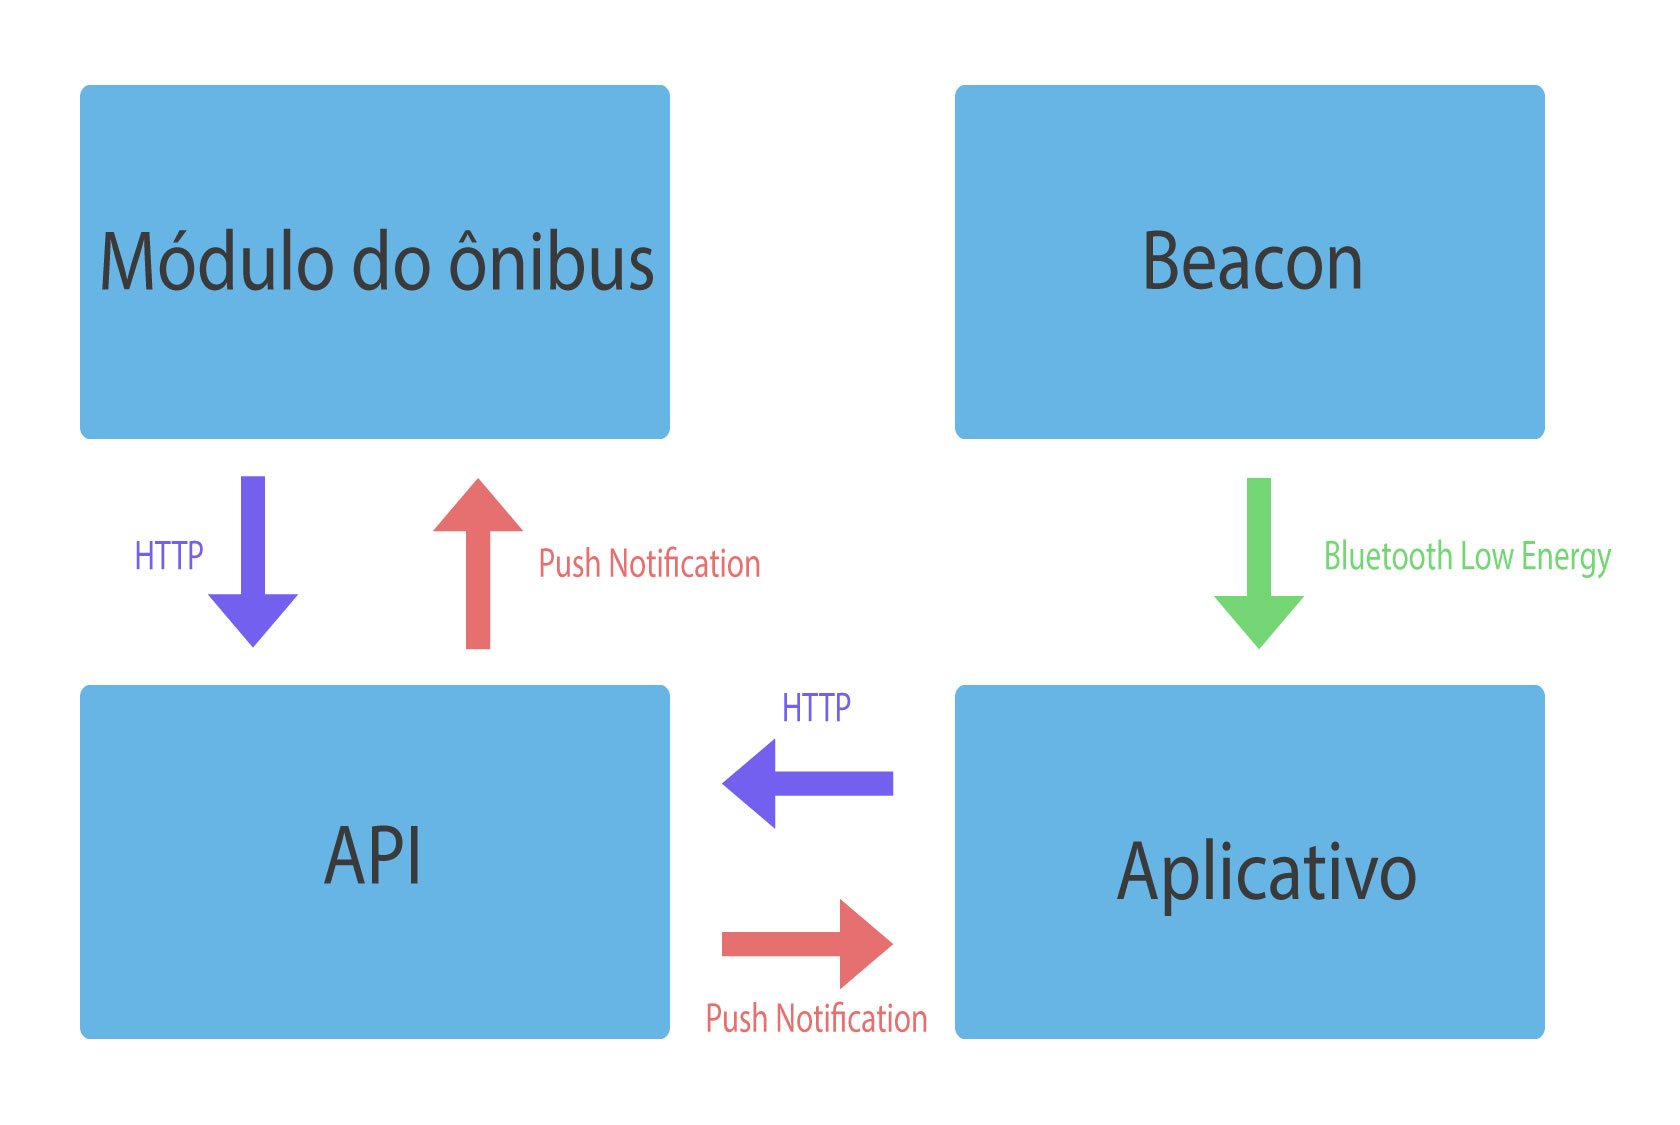
\includegraphics[width=10cm, center]{images/diagram_protocols}
\caption{Protocolos de comunicação utilizados.}
\label{Rotulo}
\end{figure}

\subsection{HTTP}

\textit{Hypertext Transfer Protocol} é um protocolo baseado em requisições. Quando um cliente necessita de uma informação, ele solicita para o servidor que retorna uma resposta. Sua especificação permite requisições do tipo \textit{GET, POST, DELETE}, dentre outros. Sua principal vantagem é não haver uma conexão aberta a todo momento para trafegar mensagens, permitindo que conexões e informações trafeguem apenas quando necessário. O formato para trafego das informações neste trabalho, por meio deste protocolo é a notação \textit{JSON}.

Para o cenário deste projeto, tanto o aplicativo quanto o módulo do ônibus estão em cenários não favoráveis para o trafego de informação em grande escala, tendo em vista a baixa qualidade das redes 3G/4G dos smartphones e das redes WiFi que possuem nos ônibus.

\subsection{Push Notification}

\textit{Push Notification} é um serviço de entrega de mensagens, parecido com \textit{SMS} (\textit{Shot Message Service}), mas que usa exclusivamente a internet para entregar. Cada plataforma possui seu próprio serviço \textit{Push}. Um bom uso deste serviço, é quando o emissor precisa enviar algo para o destinatário, sem a necessidade do destinatário ter solicitado antes, como ocorre no \textit{HTTP}.

Neste projeto temos duas situações que a tecnologia é conveniente: primeiro, existe a necessidade de avisar o motorista que é necessário, em um dado momento, parar no próximo ponto para um deficiente visual. Segundo, precisamos avisar ao deficiente visual que seu ônibus já chegou e ele pode se dirigir a ele.

Nestes dois cenários precisamos avisar os dispositivos sobre algum evento e não temos uma conexão aberta constantemente como eles. Fazendo o serviço de \textit{Push Notification} ser a melhor escolha.

Uma alternativa ao uso deste serviço são plataforma de \textit{Realtime Database}. Eles funcionam de forma parecida com o protocolo \textit{MQTT}, quando há alguma alteração em algum nó, os \textit{subscribers} são notificados sobre o novo dado.

\subsection{Bluetooth Low Energy}

O \textit{Bluetooth} é uma tecnologia de transmissão dados. Na sua versão 4.0+ ele se tornou \textit{BLE} (ou \textit{Bluetooth Smart}), trazendo a transmissão de dados com baixo consumo de energia.

Os pontos de ônibus não costumam possuir energia elétrica, com isso, surge a necessidade de uma tecnologia que tenha um moderado consumo de eletricidade. Com a necessidade do baixo consumo de energia e o envio constante, o \textit{BLE} em seu modo \textit{Beacons} ativado, se demonstrou ser a melhor alternativa suprindo todas as necessidades do projeto.

\newpage

\section{Hardware}

\subsection{Raspberry Pi 3}

\begin{figure}[!h]
\centering
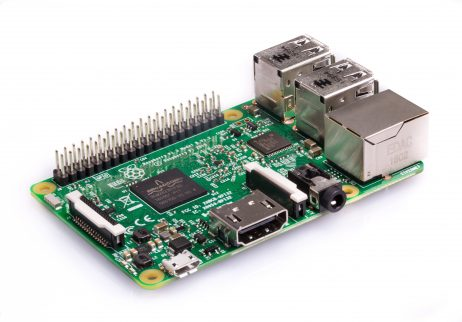
\includegraphics[width=10cm, center]{images/raspberry-pi}
\caption{Raspberry 3.}
\label{Rotulo}
\end{figure}

"A Raspberry Pi é uma máquina completa, com considerável poder de processamento, em uma placa de circuito impresso menor do que um cartão de crédito. Com ela você pode ter resultados impressionantes." (Upton, E. and Halfacree, G., 2017, Raspberry Pi - Manual do Usuário). Esta pequena placa permite ter um computador em um pequeno espaço, contando com conectividades como \textit{Bluetooth} e \textit{WiFi}, é uma excelente opção para projetos que necessitam de mais poder de processamento em um pequeno espaço. 

A Fundação Raspberry Pi, responsável pelo seu desenvolvimento, também mantém o foco da placa no meio educacional, apresentando uma plataforma acessível para que cada vez mais pessoas se interessem pelo desenvolvimento softwares.

Especificações:

\begin{itemize}
\item Quad Core 1.2GHz Broadcom BCM2837 64bit CPU
\item 1GB RAM
\item BCM43438 wireless LAN e Bluetooth Low Energy (BLE)
\item 40-pin extended GPIO
\item 4 USB 2 ports
\item 4 Pole stereo output e composite video port
\item Full size HDMI
\item CSI camera port para conectar uma câmera Raspberry Pi
\item DSI display port para conectar um display touchscreen Raspberry Pi
\item Micro SD port para carregar o sistema operacional e armazenar dados
\end{itemize}


\subsection{HM-10}

\begin{figure}[!h]
\centering
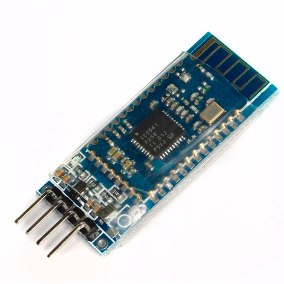
\includegraphics[width=10cm, center]{images/hm-10}
\caption{Módulo Bluetooth HM10.}
\label{Rotulo}
\end{figure}

\newpage

\subsection{Arduino Uno}

\begin{figure}[!h]
\centering
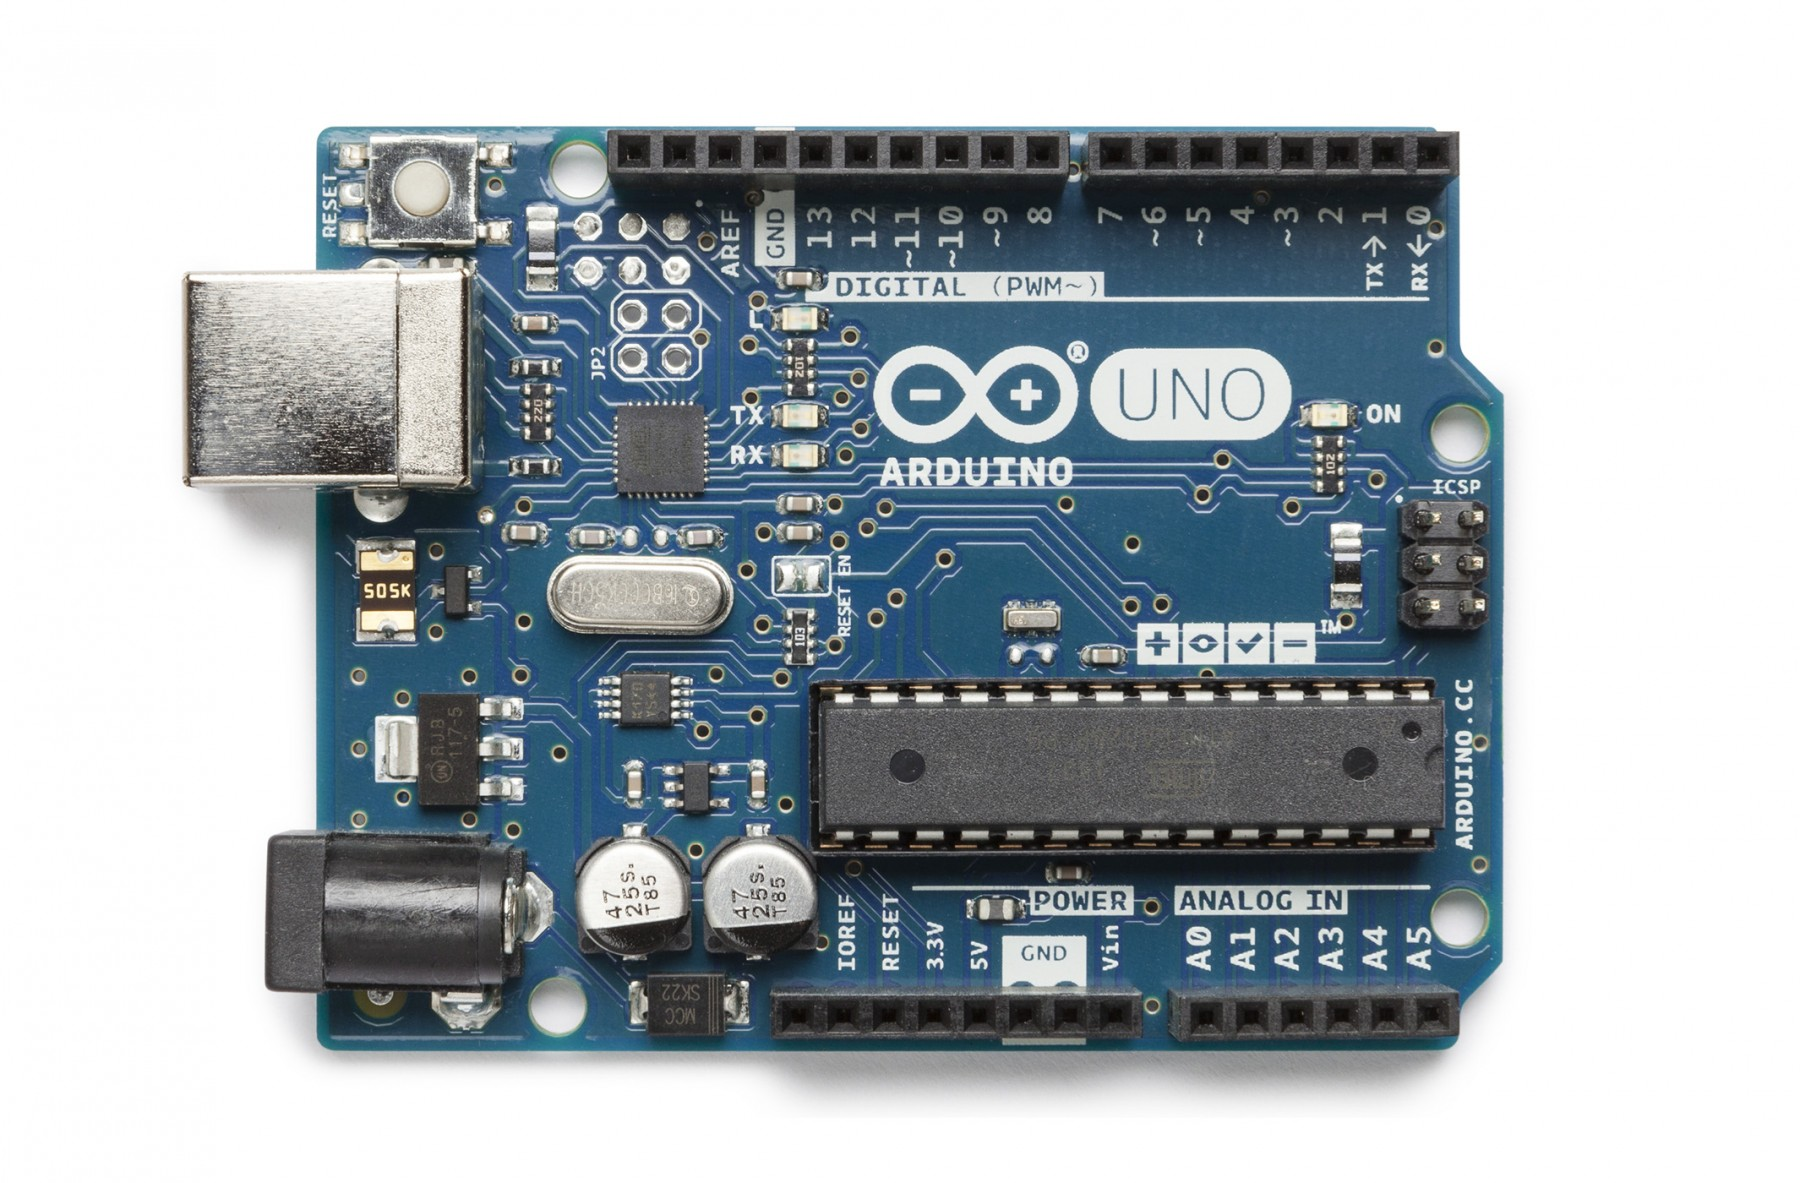
\includegraphics[width=10cm, center]{images/arduino}
\caption{Módulo Bluetooth HM10.}
\label{Rotulo}
\end{figure}

\subsection{NEO 6M}

\begin{figure}[!h]
\centering
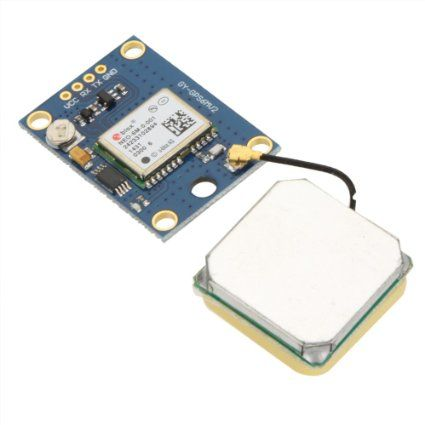
\includegraphics[width=10cm, center]{images/neo-6m}
\caption{Módulo NEO u-blox 6 GPS.}
\label{Rotulo}
\end{figure}

\textbf{Localização}

Uma característica desse módulo é trabalhar com GPS, fazendo comunicação direta com no mínimo 3 satélites para triangular sua posição com mais precisão. Alguns módulos disponíveis no mercado trabalham com A-GPS, que usam torres de telefonia móvel para conhecer sua posição.
O uso do GPS trás maior precisão, porém demora mais para estabelecer conexão com satélites. O A-GPS fornece a localização com menor tempo, porém com menor precisão e a um custo mais alto.

\textbf{Comunicação}

O módulo realiza comunicação UART (Universal Asynchronous Receiver/Transmitter), o que permite fácil comunicação com as placas utilizadas para testes.

\textbf{Preço}

Seu preço, em 08/2017, gira em torno de R\$ 60,00 e pode ser encontrado com facilidade na internet para venda. 

\section{Software}

\subsection{Sistemas Operacionais}

\subsubsection{Android}

\subsubsection{Android Things}

\subsubsection{Linguagem de Programação}

\subsection{Backend}

\subsubsection{Linguagem}

Para o desenvolvimento do \textit{web service} foi escolhida a utilização da pilha MEAN, que engloba quatro tecnologias para desenvolvimento \textit{web} que possuem como base a linguagem JavaScript.

\subsubsubsection{JavaScript}

JavaScript é uma linguagem de programação \textit{client-side}, utilizada para manipular os comportamentos de uma página, controlando o HTML e o CSS. Outra característica dela, é o fato de ser uma linguagem orientada à eventos.
Para explicar melhor o que são eventos, é importante citar que uma página HTML utiliza tags para representar seus elementos, podendo conter menus, botões e formulários, entre outros, em seu corpo. Cada elemento possui alguns atributos, sendo alguns desses chamados atributos de eventos, como por exemplo o \textit{onClick} que realiza alguma função caso o elemento referente seja clicado pelo usuário.
Para dizer as ações que devem ser tomadas quando um evento é acionado, pode-se utilizar o JavaScript. Com o decorrer do tempo, foram desenvolvidas algumas modificações em cima de JavaScript para possibilitar a utilização do mesmo no \textit{server-side}, possibilitando o desenvolvimento de um \textit{web service} em torno de uma mesma linguagem. \\

\subsubsection{MongoDB}

É um banco de dados não relacional com uma escalabilidade muito boa. Ele utiliza conceitos de \textit{collections} e \textit{documents} em sua construção. 
As \textit{collections} são equivalentes aos bancos de um ambiente que utiliza o SQL. Já os \textit{documents}, se equivalem aos registros de cada banco.
Os dados são guardados em arquivos similares aos de formato JSON (\textit{JavaScript Object Notation}).
Outro item importante sobre o MongoDB é o fato de ser \textit{schemaless}, tornando-o bem flexível em relação a inclusão de dados diferentes em uma mesma \textit{collection}, fazendo com que a validação de dados fique nas mãos dos desenvolvedores.
Apesar de \textit{schemaless}, é possível criar \textit{schemas} para auxiliar no desenvolvimento. Ao utilizar o mongoose, ferramenta desenvolvida em cima do MongoDB para trabalhar nele como se estivesse utilizando um banco relacional, é possível definir de antemão, quais os atributos que devem existir em cada \textit{collection} necessária para a aplicação.


\subsubsection{Express.js}

É um framework para Node.js que ajuda na organização de sua aplicação, caso use a arquitetura MVC, no lado do servidor. Uma de suas funções é a de facilitar a criação e manutenção de rotas, realizando uma configuração inicial com os caminhos para os \textit{controllers}, \textit{models} e \textit{views} utilizados pela sua aplicação, além de informar os dados de inicialização do servidor.


\subsubsection{Node.js}

Plataforma principal para o funcionamento da aplicação, construída sobre o motor Javascript V8 do Google Chrome.
O Node.js foi desenvolvido para construir aplicações web escaláveis de forma assíncrona, cuidando de várias conexões de maneira concorrente. Ele consegue isso através da utilização de callbacks. 
Sempre que ocorre um evento, é disparado um callback que dirá o que deve ser realizado pela aplicação. Esse processo é feito para todas as funções presentes na aplicação e sempre que houver um evento sendo disparado.
Como no lado do servidor, não existe uma interface gráfica a ser visualizada, os eventos nesse caso são dados de I/O, como algum parâmetro usado em uma busca no banco de dados, a resposta para aquele parâmetro, entre outros casos.
O Node.js é uma plataforma extremamente modularizada, com módulos criados por desenvolvedores ativos no mundo todo.
Para gerenciar esses módulos, ele utiliza o npm, responsável por instalar, atualizar ou remover suas dependências. 
É o Node.js que realiza a conexão com servidores e diz quais bancos de dados serão utilizados pela aplicação, na configuração inicial.


\subsection{Referências}

%links do HTML
\href{https://www.w3schools.com/tags/ref_eventattributes.asp}{Atributos de eventos}\\
%links do javascript
\href{http://tableless.github.io/iniciantes/manual/js/}{Guia introdutório sobre JavaScript}\\

%links do MEAN stack
ALMEIDA, Flávio. MEAN - Full stack JavaScript para aplicações web com MongoDB, Express, Angular e Node. ed. Casa do Código, 2016.\\
\href{http://nodebr.com/o-que-e-node-js/}{O que é Node.js?} %ver como fazer a referência de uma página
%links do push notifications


\chapter{Desenvolvimento}

\section{Descrição da Informação}

\subsection{Visão Geral}

\begin{figure}[!h]
\centering
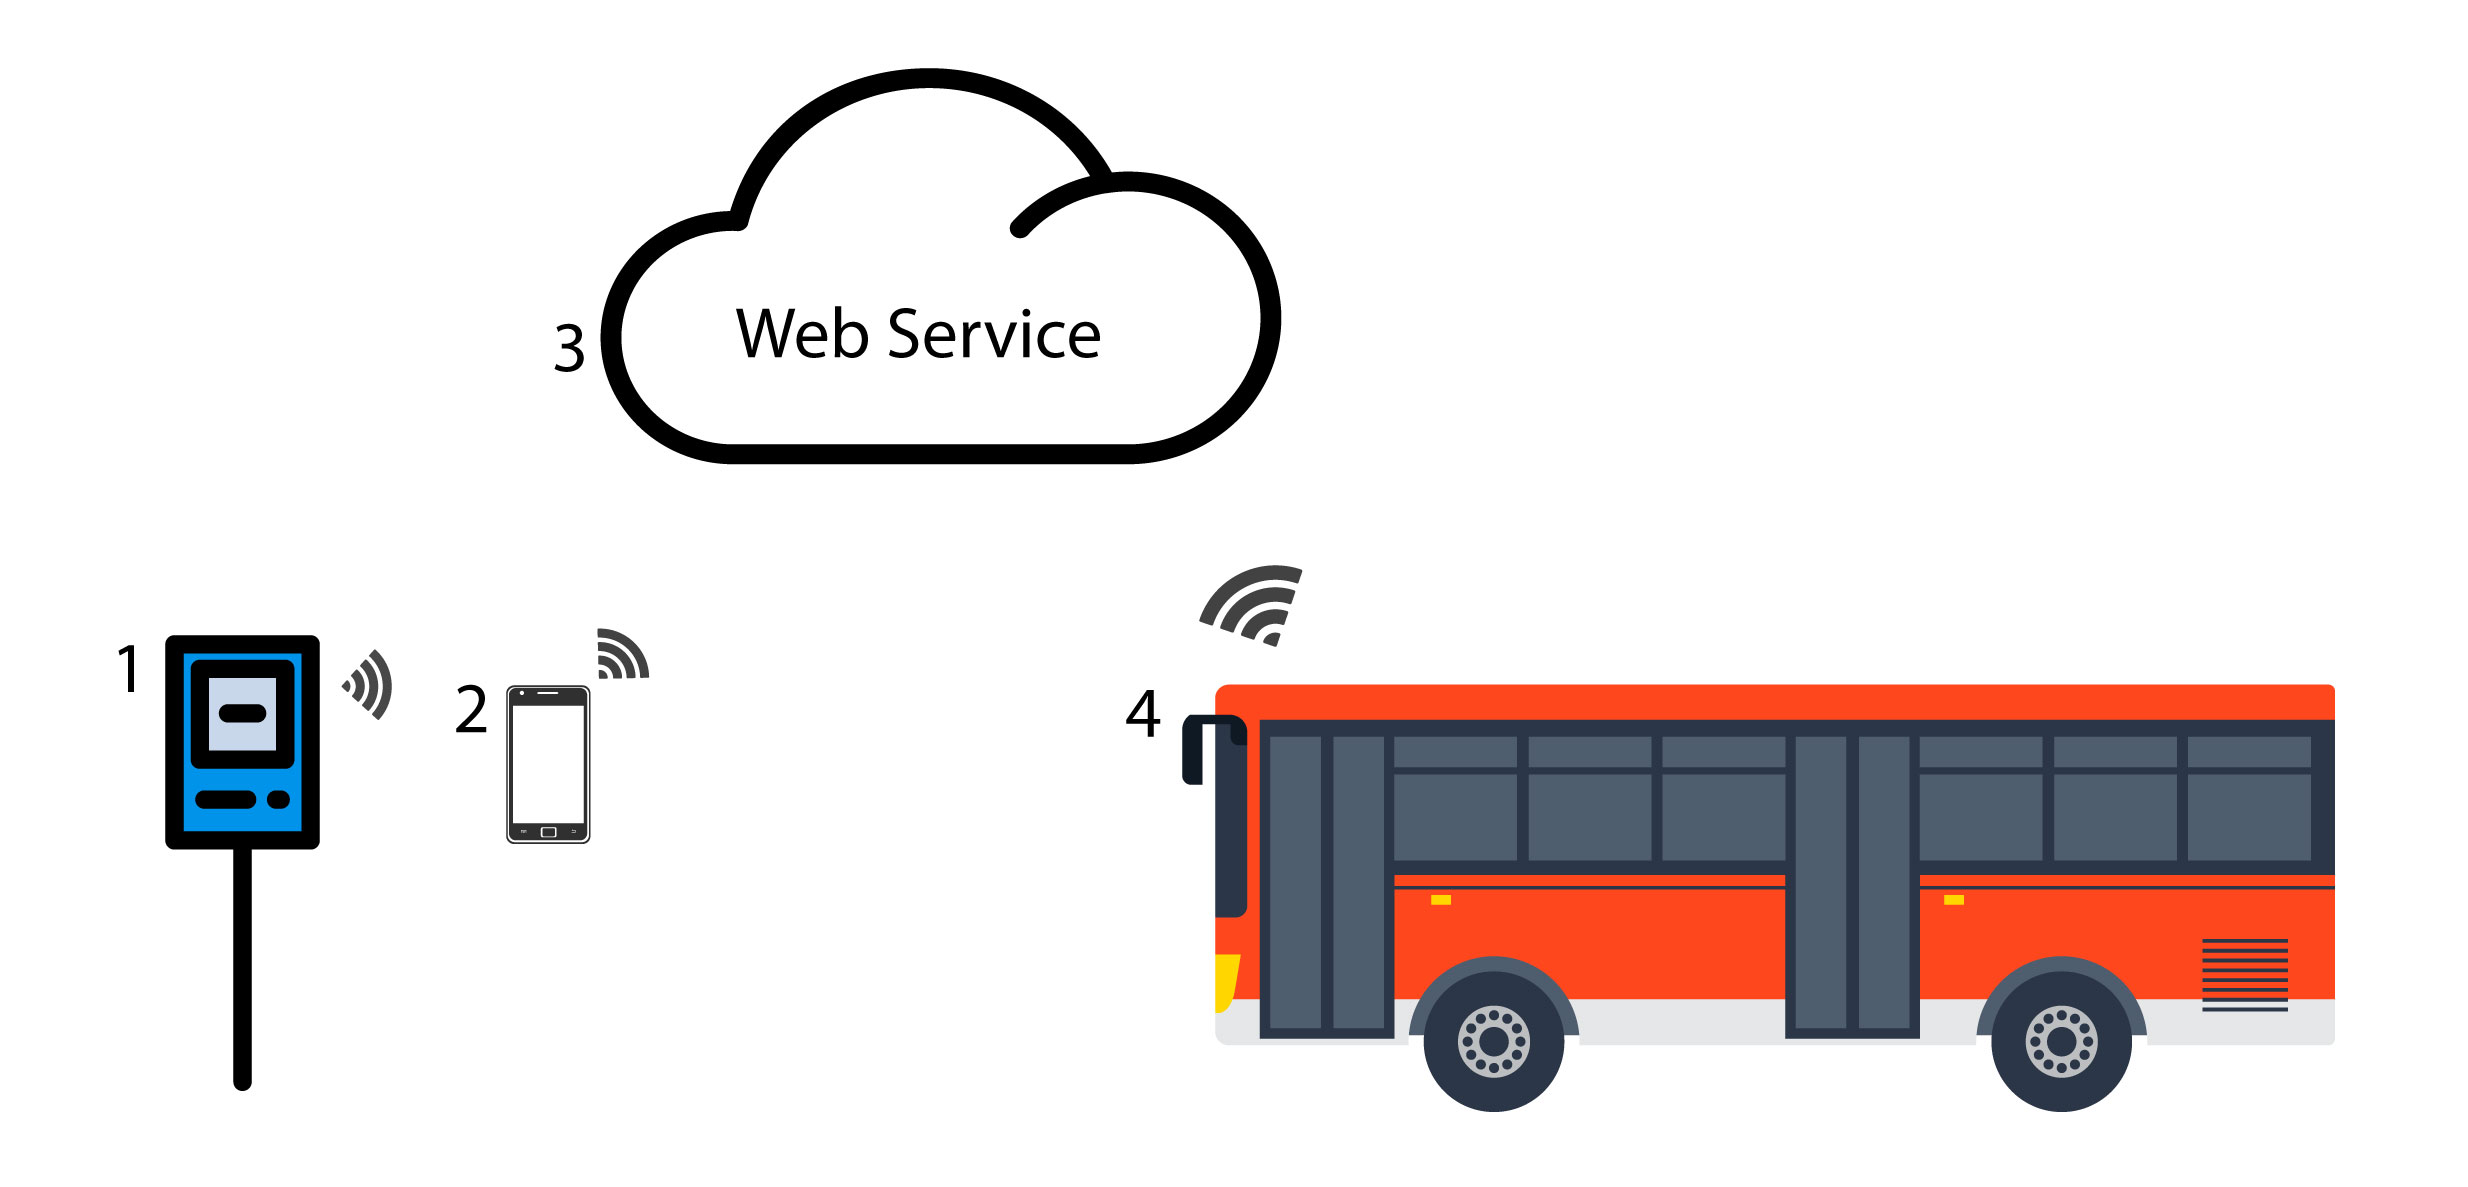
\includegraphics[width=10cm, center]{images/relations_system.jpg}
\caption{Visão geral da comunicação dos componentes.}
\label{Rotulo}
\end{figure}

\begin{description}
\item[1. Módulo da parada de ônibus:] Emite informações de identificação da parada.

\item[2. Aplicativo:] Reconhece o ponto de ônibus e solicita informações da API.

\item[3. API:] Intermediário entre o aplicativo e o módulo do ônibus.

\item[4. Módulo do Ônibus:] Mantém constante comunicação com o \textit{Web Service} enviando dados de geolocalização. Recebe também informação se deve alertar o motorista sobre deficiente visual na próxima parada.
\end{description}

\newpage

\subsection{Representação do Fluxo da Informação}

\begin{figure}[!h]
\centering
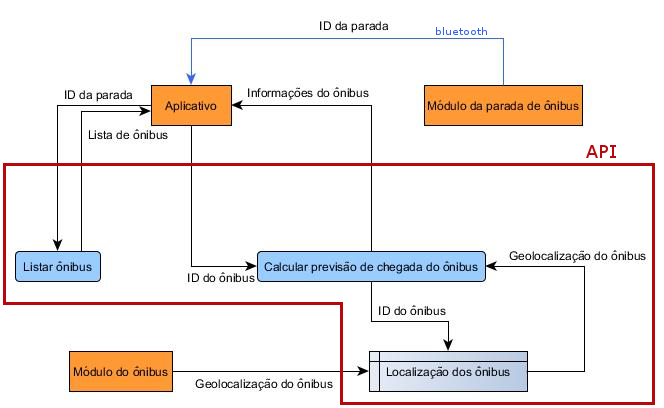
\includegraphics[width=10cm, center]{images/data-flux.png}
\caption{Diagrama de fluxo de dados.}
\label{Rotulo}
\end{figure}

\begin{figure}[!h]
\centering
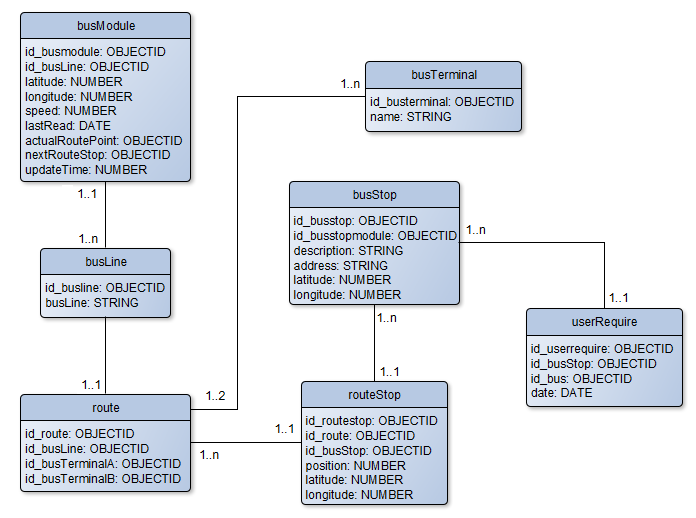
\includegraphics[width=10cm, center]{images/database-api.png}
\caption{Diagrama de banco de dados.}
\label{Rotulo}
\end{figure}

\newpage

\subsection{Descrição Funcional}

\subsubsection{Aplicativo para dispositivo móvel}

Aplicativo que irá interagir com o deficiente visual. Sua função é verificar qual Beacon está mais próximo para que a API possa saber sua localização, podendo listar, via interface áudio-visual, para o usuário, quais linhas passam no ponto de parada que ele está.

\subsubsection{API}

Sistema que recebe informações do aplicativo e do módulo do ônibus. Tem como objetivo acessar os dados gravados no banco de dados para que possa prover informações de previsão ao aplicativo. Também é responsável por verificar se o módulo do ônibus deve alertar a presença de um usuário no próximo ponto. Além de calcular a previsão de um ônibus até o ponto de parada selecionado.

\subsubsection{Módulo do ponto de ônibus}

Dispositivo localizado em um determinado ponto de parada de ônibus. Emite constantemente um sinal ID para a identificação do ponto que ele se refere.

\subsubsection{Módulo do ônibus}

Dispositivo instalado no ônibus. Mantém comunicação constante com a API para informar sua geolocalização. Verifica ao mesmo tempo a necessidade de alertar o motorista se existe um deficiente visual aguardando no próximo ponto de parada.

\newpage

\subsection{Interfaces com Sistema}

\subsubsection{Aplicativo}

\subsubsubsection{Busca por um ponto próximo}

\begin{figure}[!h]
\centering
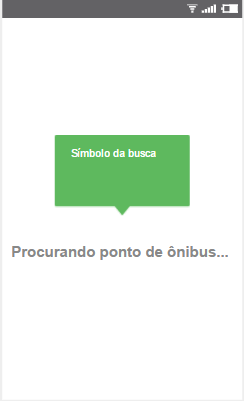
\includegraphics[width=5cm, center]{images/tela-1-buscando-beacon.PNG}
\caption{Tela do aplicativo ao buscar por um ponto de ônibus próximo.}
\label{Rotulo}
\end{figure}

\begin{table}[!h]
\centering
\begin{tabular}{@{}|c|c|c|c|c|@{}}
\hline
Número & 
Nome & 
Descrição & 
Requisitos & 
Grupo\\ \hline
1 & \begin{tabular}[c]{@{}c@{}}Símbolo da busca \\ do ponto de ônibus\end{tabular} & \begin{tabular}[c]{@{}c@{}}Indica que o aplicativo \\ está procurando um \\ ponto de ônibus\end{tabular}                  & -                     & Imagem e texto \\ \hline
2 & Áudio sobre busca & \begin{tabular}[c]{@{}c@{}}Indica ao usuário que \\ está sendo feito uma \\ busca por algum \\ ponto próximo\end{tabular} & Função Talkback ativa & Áudio\\ \hline
\end{tabular}
\caption{Descrição dos elementos da tela de busca por ponto de ônibus próximo.}
\label{Rotulo}
\end{table}

\newpage

\subsubsubsection{Busca por um ponto na API}

\begin{figure}[!h]
\centering
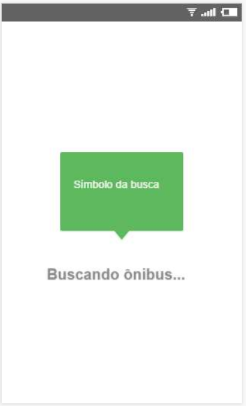
\includegraphics[width=5cm, center]{images/tela-2-buscando-ponto.PNG}
\caption{Tela do aplicativo ao buscar por um ponto de ônibus na API.}
\label{Rotulo}
\end{figure}

\begin{table}[!h]
\centering
\begin{tabular}{@{}|c|c|c|c|c|@{}}
\hline
Número & 
Nome & 
Descrição & 
Requisitos & 
Grupo\\ \hline
1 & \begin{tabular}[c]{@{}c@{}}Símbolo da busca \\ das linhas de ônibus\end{tabular} & \begin{tabular}[c]{@{}c@{}}Indica que o \\ aplicativo \\ procura as\\linhas de ônibus\end{tabular} & \begin{tabular}[c]{@{}c@{}}O sistema deve ter\\detectado um ponto\\de ônibus\end{tabular} & Imagem e texto \\ \hline
2 & Áudio sobre busca & \begin{tabular}[c]{@{}c@{}}Indica ao usuário\\ que está sendo \\feito uma busca\\ dos ônibus disponíveis\end{tabular} & Função Talkback ativa & Áudio\\ \hline
\end{tabular}
\caption{Descrição dos elementos da tela de busca por ponto de ônibus na API.}
\label{Rotulo}
\end{table}

\newpage

\subsubsubsection{Lista de ônibus disponíveis}

\begin{figure}[!h]
\centering
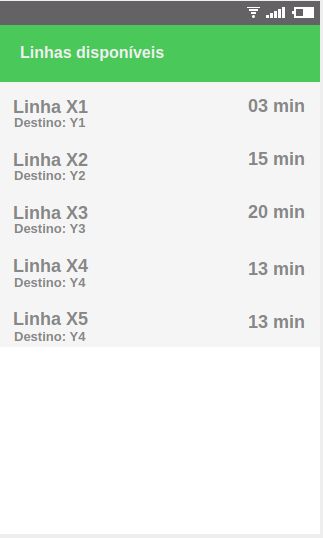
\includegraphics[width=5cm, center]{images/tela-3-lista-de-onibus.PNG}
\caption{Tela do aplicativo com ônibus disponíveis.}
\label{Rotulo}
\end{figure}

\begin{table}[!h]
\centering
\begin{tabular}{@{}|c|c|c|c|c|@{}}
\hline
Número & 
Nome & 
Descrição & 
Requisitos & 
Grupo\\ \hline
1 & Lista de linhas & \begin{tabular}[c]{@{}c@{}}Lista de linhas\\ que o usuário\\ pode escolher\end{tabular} & \begin{tabular}[c]{@{}c@{}}Ter recebido uma\\ lista da API\end{tabular} & Botão \\ \hline
2 & \begin{tabular}[c]{@{}c@{}}Áudio sobre escolha\\ de um item\end{tabular} & \begin{tabular}[c]{@{}c@{}}Indica que a lista\\ de ônibus já está\\ disponível\end{tabular} & Função Talkback ativa & Áudio\\ \hline
\end{tabular}
\caption{Descrição dos elementos da tela de busca por ponto de ônibus na API.}
\label{Rotulo}
\end{table}

\newpage

\subsubsubsection{Detalhes do ônibus}

\begin{figure}[!h]
\centering
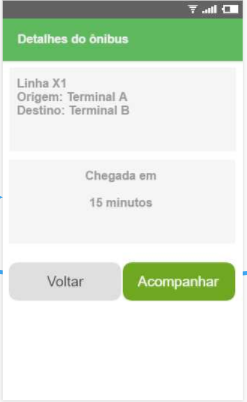
\includegraphics[width=5cm, center]{images/tela-4-informacoes-do-onibus.PNG}
\caption{Tela do aplicativo com detalhes de um ônibus.}
\label{Rotulo}
\end{figure}

\begin{table}[!h]
\centering
\begin{tabular}{@{}|c|c|c|c|c|@{}}
\hline
Número                  & Nome                                  & Descrição                                                                                                                                     & Requisitos                                                                              & Grupo                      \\ \hline
\multicolumn{1}{|c|}{1} & \multicolumn{1}{c|}{Linha X1}         & \multicolumn{1}{c|}{Mostra a linha selecionada}                                                                                               & \multicolumn{1}{c|}{\begin{tabular}[c]{@{}c@{}}Receber previsão \\ da API\end{tabular}} & \multicolumn{1}{c|}{Texto} \\ \hline
\multicolumn{1}{|c|}{2} & \multicolumn{1}{c|}{Origem}           & \multicolumn{1}{c|}{Exibe o ponto inicial da linha}                                                                                           & \multicolumn{1}{c|}{\begin{tabular}[c]{@{}c@{}}Receber previsão \\ da API\end{tabular}} & \multicolumn{1}{c|}{Texto} \\ \hline
\multicolumn{1}{|c|}{3} & \multicolumn{1}{c|}{Destino}          & \multicolumn{1}{c|}{Exibe o ponto final da linha}                                                                                             & \multicolumn{1}{c|}{\begin{tabular}[c]{@{}c@{}}Receber previsão \\ da API\end{tabular}} & \multicolumn{1}{c|}{Texto} \\ \hline
\multicolumn{1}{|c|}{4} & \multicolumn{1}{c|}{Chegada em}       & \multicolumn{1}{c|}{\begin{tabular}[c]{@{}c@{}}Exibe a previsão de\\  chegada da linha\end{tabular}}                                          & \multicolumn{1}{c|}{\begin{tabular}[c]{@{}c@{}}Receber previsão \\ da API\end{tabular}} & \multicolumn{1}{c|}{Texto} \\ \hline
\multicolumn{1}{|c|}{5} & \multicolumn{1}{c|}{Voltar}           & \multicolumn{1}{c|}{Volta para a seleção de linhas}                                                                                           & \multicolumn{1}{c|}{\begin{tabular}[c]{@{}c@{}}Receber previsão\\  da API\end{tabular}} & \multicolumn{1}{c|}{Botão} \\ \hline
\multicolumn{1}{|c|}{6} & \multicolumn{1}{c|}{Solicitar ônibus} & \multicolumn{1}{c|}{\begin{tabular}[c]{@{}c@{}}Solicita que o ônibus\\  pare no seu\\  ponto e acionar o \\ acompanhamento dele\end{tabular}} & \multicolumn{1}{c|}{\begin{tabular}[c]{@{}c@{}}Receber previsão \\ da API\end{tabular}} & \multicolumn{1}{c|}{Botão} \\ \hline
7                       & Áudio sobre previsão                  & \begin{tabular}[c]{@{}c@{}}Alerta ao usuário a\\  previsão do ônibus\end{tabular}                                                             & \begin{tabular}[c]{@{}c@{}}Receber previsão \\ da API\end{tabular}                      & Áudio                      \\ \hline
\end{tabular}
\caption{Descrição dos elementos da tela de detalhes do ônibus.}
\label{Rótulo}
\end{table}

\newpage

\subsubsubsection{Aguardando um ônibus}

\begin{figure}[!h]
\centering
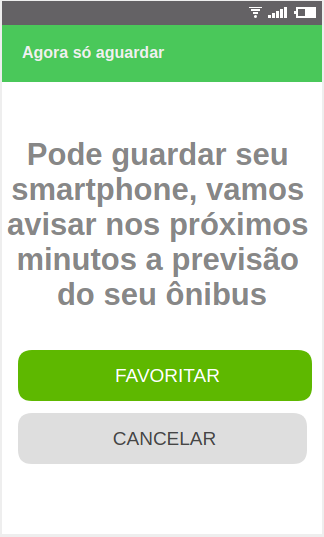
\includegraphics[width=5cm, center]{images/tela-5-acompanhamento-do-onibus.PNG}
\caption{Tela do aplicativo sobre a solicitação de um ônibus.}
\label{Rotulo}
\end{figure}

\begin{table}[!h]
\centering
\begin{tabular}{|c|c|c|c|c|}
\hline
Número & Nome                                                                    & Descrição                                                                                                              & Requisitos                                                                                                                              & Grupo \\ \hline
1
 & \begin{tabular}[c]{@{}c@{}}Informação \\ de previsão\end{tabular}       & \begin{tabular}[c]{@{}c@{}}O sistema irá \\ informar o \\ usuário até a \\ chegada do ônibus\end{tabular}              & \begin{tabular}[c]{@{}c@{}}Ter selecionado botão \\ Solicitar ônibus\end{tabular}                                                       & Texto \\ \hline
2      & Favoritar                                                               & \begin{tabular}[c]{@{}c@{}}Adiciona ônibus\\ como favorito\end{tabular}                                                & \begin{tabular}[c]{@{}c@{}}O ônibus não pode \\ estar cadastrado \\ como favorito. \\ Caso esteja o \\ botão não é exibido\end{tabular} & Botão \\ \hline
3      & Cancelar                                                                & \begin{tabular}[c]{@{}c@{}}Cancela o acompanhamento \\ do ônibus e solicita \\ que não pare mais no ponto\end{tabular} & \begin{tabular}[c]{@{}c@{}}Ter selecionado botão\\  Solicitar ônibus\end{tabular}                                                       & Botão \\ \hline
4      & \begin{tabular}[c]{@{}c@{}}Áudio sobre o \\ acompanhamento\end{tabular} & \begin{tabular}[c]{@{}c@{}}Informa ao usuário \\ que está sendo \\ feito o acompanhamento \\ do ônibus\end{tabular}    & \begin{tabular}[c]{@{}c@{}}Ter escolhido acompanhar \\ um ônibus.\\ Função Talkback ativa\end{tabular}                                  & Áudio \\ \hline
\end{tabular}
\caption{Descrição dos elementos da tela sobre a solicitação de um ônibus.}
\label{Rótulo}
\end{table}

\newpage

\subsubsection{Módulo do ônibus}

\subsubsubsection{Carregando Informações}

\begin{figure}[!h]
\centering
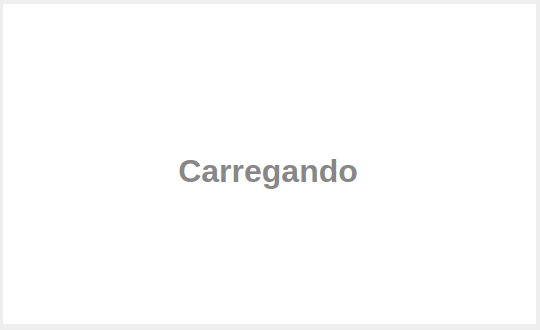
\includegraphics[width=10cm, center]{images/busmodule-carregando}
\caption{Tela do módulo do ônibus quando está carregando informações.}
\label{Rotulo}
\end{figure}

\begin{table}[!h]
\centering
\begin{tabular}{|c|c|c|c|c|}
\hline
Número & Nome                                                                    & Descrição                                                                                                              & Requisitos                                                                                                                              & Grupo \\ 
\hline 
\begin{tabular}[c]{@{}c@{}}1\end{tabular}  & \begin{tabular}[c]{@{}c@{}}Mensagem\end{tabular}  & \begin{tabular}[c]{@{}c@{}}Informa que está carregando informações \\do servidor\end{tabular}  & \begin{tabular}[c]{@{}c@{}}Ter iniciado o sistema\end{tabular}  & \begin{tabular}[c]{@{}c@{}}Texto\end{tabular}  \\ 
\hline 
\end{tabular} 
\caption{Descrição dos elementos da tela sobre estar carregando informações.}
\label{Rótulo}
\end{table}

\newpage

\subsubsubsection{Aguardando iniciar a rota}

\begin{figure}[!h]
\centering
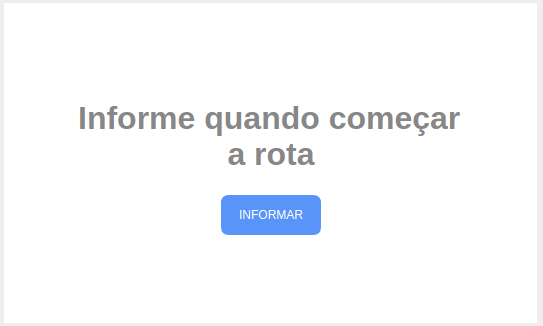
\includegraphics[width=10cm, center]{images/busmodule-comecar-rota}
\caption{Tela do módulo do ônibus aguardando motorista inicar rota.}
\label{Rotulo}
\end{figure}

\begin{table}[!h]
\centering
\begin{tabular}{|c|c|c|c|c|}
\hline
Número & Nome                                                                    & Descrição                                                                                                              & Requisitos                                                                                                                              & Grupo \\
\hline 
\begin{tabular}[c]{@{}c@{}}1\end{tabular} 
& \begin{tabular}[c]{@{}c@{}}Informação para\\ começar rota\end{tabular} 
& \begin{tabular}[c]{@{}c@{}}Informar que precisa avisar \\ quando começar a rota\end{tabular} 
& \begin{tabular}[c]{@{}c@{}}-\end{tabular} & \begin{tabular}[c]{@{}c@{}}Texto\end{tabular} \\ 
\hline 
\begin{tabular}[c]{@{}c@{}}2\end{tabular} 
& \begin{tabular}[c]{@{}c@{}}Começar rota\end{tabular} 
& \begin{tabular}[c]{@{}c@{}}Começar rotina de envio da posição\end{tabular} 
& \begin{tabular}[c]{@{}c@{}}-\end{tabular} 
& \begin{tabular}[c]{@{}c@{}}Botão\end{tabular} \\ 
\hline 
\end{tabular} 
\caption{Descrição dos elementos da tela sobre começar uma rota.}
\label{Rótulo}
\end{table}

\newpage

\subsubsubsection{Realizando uma rota}

\begin{figure}[!h]
\centering
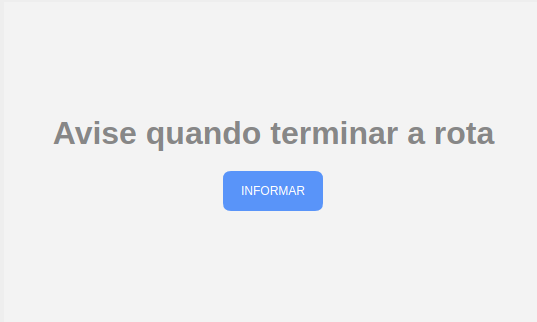
\includegraphics[width=10cm, center]{images/busmodule-finish-route}
\caption{Tela do módulo do ônibus quando motorista está fazendo a rota.}
\label{Rotulo}
\end{figure}

\begin{table}[!h]
\centering
\begin{tabular}{|c|c|c|c|c|}
\hline
Número & Nome                                                                    & Descrição                                                                                                              & Requisitos                                                                                                                              & Grupo \\
\hline 
\begin{tabular}[c]{@{}c@{}}1\end{tabular} 
& \begin{tabular}[c]{@{}c@{}}Informação sobre\\termino da rota\end{tabular} 
& \begin{tabular}[c]{@{}c@{}}Informar que precisa avisar \\ quando terminar a rota\end{tabular} 
& \begin{tabular}[c]{@{}c@{}}Ter iniciado\\uma rota\end{tabular} & \begin{tabular}[c]{@{}c@{}}Texto\end{tabular} \\ 
\hline 
\begin{tabular}[c]{@{}c@{}}2\end{tabular} 
& \begin{tabular}[c]{@{}c@{}}Terminar rota\end{tabular} 
& \begin{tabular}[c]{@{}c@{}}Terminar rotina de envio da posição\end{tabular} 
& \begin{tabular}[c]{@{}c@{}}Ter iniciado\\uma rota\end{tabular} 
& \begin{tabular}[c]{@{}c@{}}Botão\end{tabular} \\ 
\hline 
\end{tabular} 
\caption{Descrição dos elementos da tela sobre terminar uma rota.}
\label{Rótulo}
\end{table}

\newpage

\subsubsubsection{Aviso para parar no próximo ponto}

\begin{figure}[!h]
\centering
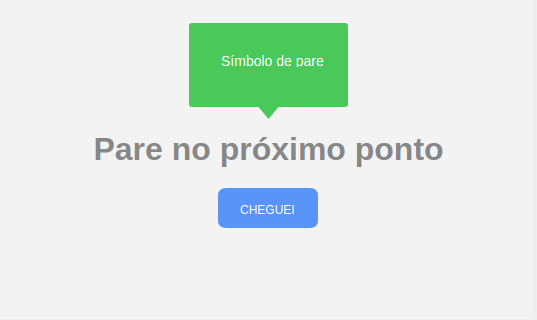
\includegraphics[width=10cm, center]{images/busmodule-pare}
\caption{Tela do módulo do ônibus quando motorista precisar parar no próximo ponto.}
\label{Rotulo}
\end{figure}

\begin{table}[!h]
\centering
\begin{tabular}{|c|c|c|c|c|}
\hline
Número & Nome                                                                    & Descrição                                                                                                              & Requisitos                                                                                                                              & Grupo \\
\hline 
\begin{tabular}[c]{@{}c@{}}1\end{tabular} 
& \begin{tabular}[c]{@{}c@{}}Simbolo de alerta\\ para parar\end{tabular} 
& \begin{tabular}[c]{@{}c@{}}Informar que precisa parar \\ no próximo ponto\end{tabular} 
& \begin{tabular}[c]{@{}c@{}}Servidor informar\\ a necessidade\end{tabular} & \begin{tabular}[c]{@{}c@{}}Imagem e Texto\end{tabular} \\ 
\hline 
\begin{tabular}[c]{@{}c@{}}2\end{tabular} 
& \begin{tabular}[c]{@{}c@{}}Informar chegada\end{tabular} 
& \begin{tabular}[c]{@{}c@{}}Envia informação que\\ chegou no ponto\end{tabular} 
& \begin{tabular}[c]{@{}c@{}}Ter chegado no\\ ponto\end{tabular} 
& \begin{tabular}[c]{@{}c@{}}Botão\end{tabular} \\ 
\hline 
\end{tabular} 
\caption{Descrição dos elementos da tela sobre terminar uma rota.}
\label{Rótulo}
\end{table}

\newpage

\subsection{Casos de Uso}

\begin{figure}[!h]
\centering
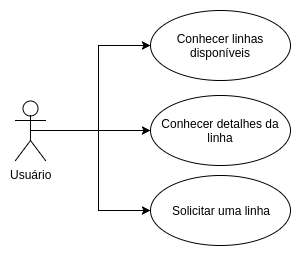
\includegraphics[width=6cm, center]{images/use-case-diagram.png}
\caption{Diagrama de caso de uso.}
\label{Rotulo}
\end{figure}

\subsubsection{Narrativas: Casos de Uso}

Solicitar horário do próximo ônibus da linha e sentido escolhido: Este caso de uso acontece quando um usuário solicita qual será a previsão de horário do próximo ônibus, de uma linha e sentido que ele poderá escolher de acordo com o seu ponto de ônibus.

Solicitar parada do ônibus escolhido: Este caso de uso é uma extensão do caso de uso “Solicitar horário do próximo ônibus da linha e sentido escolhido”, onde depois de escolher uma linha e sentido ele poderá solicitar a parada do próximo ônibus escolhido.

\newpage

\subsubsection{Diagramas de apoio para compreensão funcional}

\bgroup
\def\arraystretch{1.5}
\begin{table}[!h]
\centering
\begin{tabular}{|l|l|}
\hline
\multicolumn{2}{|l|}{\textbf{Identificação:} UC001}                                                                 \\ \hline
\multicolumn{2}{|l|}{\textbf{Nome:} Solicitar horário do próximo ônibus}                                            \\ \hline
\multicolumn{2}{|l|}{\textbf{Atores:} Usuário}                                                                      \\ \hline
\multicolumn{2}{|l|}{\textbf{Pré-condições:} O aplicativo precisa ter lido o ID do módulo do ponto de ônibus}       \\ \hline
\multicolumn{2}{|l|}{\textbf{Pós-condições:} Retorno do horário do próximo ônibus e da solicitação de parada}       \\ \hline
\multicolumn{2}{|c|}{\textbf{Fluxo de eventos}}                                                           \\ \hline
\textbf{Ator}                       & \textbf{Sistema}                                                    \\ \hline
\begin{tabular}[c]{@{}l@{}}1. Usuário chega ao ponto de ônibus\end{tabular} & \begin{tabular}[c]{@{}l@{}}2. Sistema lê o ID do ponto de ônibus \\e retorna uma lista de linhas\end{tabular} \\ \hline
\begin{tabular}[c]{@{}l@{}}3. Usuário escolhe uma linha\end{tabular}        & \begin{tabular}[c]{@{}l@{}}4. Informar constantemente \\o horário do ônibus\end{tabular}                      \\ \hline
\multicolumn{2}{|c|}{\textbf{Fluxo alternativo}}                                                          \\ \hline
\multicolumn{2}{|l|}{Não possui fluxo alternativo}                                                        \\ \hline
\end{tabular}
\caption{Tabela com caso de uso UC001.}
\label{Rótulo}
\end{table}
\egroup

\bgroup
\def\arraystretch{1.5}
\begin{table}[!h]
\centering
\begin{tabular}{|l|l|}
\hline
\multicolumn{2}{|l|}{\textbf{Identificação:} UC002}                                                                                                                                                                    \\ \hline
\multicolumn{2}{|l|}{\textbf{Nome:} Solicitar parada do ônibus escolhido}                                                                                                                                              \\ \hline
\multicolumn{2}{|l|}{\textbf{Atores:} Usuário}                                                                                                                                                                         \\ \hline
\multicolumn{2}{|l|}{\textbf{Pré-condições:} O usuário precisa ter solicitado o ônibus de uma linha}                                                                                                                   \\ \hline
\multicolumn{2}{|l|}{\textbf{Pós-condições:} Confirmação de parada}                                                                                                                                                    \\ \hline
\multicolumn{2}{|c|}{\textbf{Fluxo de eventos}}                                                                                                                                                                       \\ \hline
\textbf{Ator}                                                                                              & \textbf{Sistema} \\ \hline
\begin{tabular}[c]{@{}l@{}}1. Usuário confirma solicitação \\ de parada no seu ponto\end{tabular} & \begin{tabular}[c]{@{}l@{}}2. Sistema retorna tela de seleção\\  de ponto de ônibus destino\end{tabular} \\ \hline
\multicolumn{2}{|l|}{\textbf{Fluxo alternativo}}                                                                                                                                                                      \\ \hline
\begin{tabular}[c]{@{}l@{}}1.a 1. Usuário cancela \\ solicitação de parada\end{tabular}           & 2. Sistema retorna cancela operação                                                                      \\ \hline
\begin{tabular}[c]{@{}l@{}}3.a 1. Usuário cancela\\  escolha de ponto de ônibus\end{tabular}      & 2. Sistema retorna cancela operação                                                                      \\ \hline
\end{tabular}
\caption{Tabela com caso de uso UC002.}
\label{Rótulo}
\end{table}
\egroup

\newpage

\begin{figure}[!h]
\centering
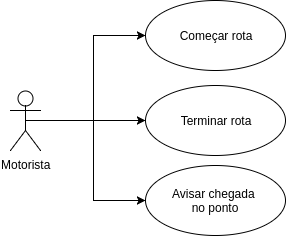
\includegraphics[width=6cm, center]{images/use-case-bus-module.png}
\caption{Diagrama de caso de uso.}
\label{Rotulo}
\end{figure}

\subsubsection{Narrativas: Casos de Uso}

Iniciar uma rota: Este caso de uso acontece quando o motorista inicia sua rota e precisa informar isso ao módulo, para que o dispositivo comece a enviar seus dados de geolocalização para o \textit{web service}.

Terminar uma rota: Este caso de uso acontece quando o motorista termina a rota do ônibus e precisa informar isso ao módulo, para que o dispositivo pare de enviar seus dados de geolocalização para o \textit{web service}.

Avisar chegada no ponto: Este caso de uso acontece quando um deficiente visual solicitou o ônibus e o motorista está parado no ponto de ônibus. Quando motorista avisa que chegou, é disparado um alerta para o deficiente visual.

\newpage

\subsubsection{Diagramas de apoio para compreensão funcional}

\bgroup
\def\arraystretch{1.5}
\begin{table}[!h]
\centering
\begin{tabular}{|l|l|}
\hline
\multicolumn{2}{|l|}{\textbf{Identificação:} UC003}                                                                                                                                                                    \\ \hline
\multicolumn{2}{|l|}{\textbf{Nome:} Iniciar uma rota}                                                                                                                                              \\ \hline
\multicolumn{2}{|l|}{\textbf{Atores:} Motorista}                                                                                                                                                                         \\ \hline
\multicolumn{2}{|l|}{\textbf{Pré-condições:} O motorista precisa ter iniciado o módulo}                                                                                                                   \\ \hline
\multicolumn{2}{|l|}{\textbf{Pós-condições:} -}                                                                                                                                                    \\ \hline
\multicolumn{2}{|c|}{\textbf{Fluxo de eventos}}                                                                                                                                                                       \\ \hline
\textbf{Ator}                                                                                              & \textbf{Sistema} \\ \hline
\begin{tabular}[c]{@{}l@{}}1. Usuário confirma o inicio \\da rota\end{tabular} 
& \begin{tabular}[c]{@{}l@{}}2. Módulo começa a enviar dados\\ de geolocalização\end{tabular} 
\\ \hline
 & \begin{tabular}[c]{@{}l@{}}3. Sistema exibe tela com opção \\de parar envio de dados\end{tabular}  \\ \hline
\end{tabular}
\caption{Tabela com caso de uso UC003.}
\label{Rótulo}
\end{table}
\egroup

\bgroup
\def\arraystretch{1.5}
\begin{table}[!h]
\centering
\begin{tabular}{|l|l|}
\hline
\multicolumn{2}{|l|}{\textbf{Identificação:} UC004}                                                                                                                                                                    \\ \hline
\multicolumn{2}{|l|}{\textbf{Nome:} Finalizar uma rota}                                                                                                                                              \\ \hline
\multicolumn{2}{|l|}{\textbf{Atores:} Motorista}                                                                                                                                                                         \\ \hline
\multicolumn{2}{|l|}{\textbf{Pré-condições:} O motorista precisa ter iniciado uma rota}                                                                                                                   \\ \hline
\multicolumn{2}{|l|}{\textbf{Pós-condições:} -}                                                                                                                                                    \\ \hline
\multicolumn{2}{|c|}{\textbf{Fluxo de eventos}}                                                                                                                                                                       \\ \hline
\textbf{Ator}                                                                                              & \textbf{Sistema} \\ \hline
\begin{tabular}[c]{@{}l@{}}1. Motorista confirma o fim \\da rota\end{tabular} 
& \begin{tabular}[c]{@{}l@{}}2. Módulo para de enviar dados\\ de geolocalização\end{tabular} 
\\ \hline
 & \begin{tabular}[c]{@{}l@{}}3. Sistema exibe tela com opção \\de iniciar envio de dados\end{tabular}  \\ \hline
\end{tabular}
\caption{Tabela com caso de uso UC004.}
\label{Rótulo}
\end{table}
\egroup

\newpage

\bgroup
\def\arraystretch{1.5}
\begin{table}[!h]
\centering
\begin{tabular}{|l|l|}
\hline
\multicolumn{2}{|l|}{\textbf{Identificação:} UC005}                                                                                                                                                                    \\ \hline
\multicolumn{2}{|l|}{\textbf{Nome:} Avisar chegada no ponto}                                                                                                                                              \\ \hline
\multicolumn{2}{|l|}{\textbf{Atores:} Motorista}                                                                                                                                                                         \\ \hline
\multicolumn{2}{|l|}{\textbf{Pré-condições:} O motorista precisa ter iniciado uma rota}                                                                                                                   \\ \hline
\multicolumn{2}{|l|}{\textbf{Pós-condições:} -}                                                                                                                                                    \\ \hline
\multicolumn{2}{|c|}{\textbf{Fluxo de eventos}}                                                                                                                                                                       \\ \hline
\textbf{Ator}                                                                                              & \textbf{Sistema} \\ \hline
\begin{tabular}[c]{@{}l@{}}1. Motorista confirma chegada no \\ponto de ônibus\end{tabular} 
& \begin{tabular}[c]{@{}l@{}}2. Módulo enviar aviso\\ de chegada\end{tabular} 
\\ \hline
 & \begin{tabular}[c]{@{}l@{}}3. Sistema exibe tela com opção \\de parar envio de dados\end{tabular}  \\ \hline
\end{tabular}
\caption{Tabela com caso de uso UC005.}
\label{Rótulo}
\end{table}
\egroup

\newpage

\section{Módulo do Ponto de Ônibus}

\subsection{Hardware}

\begin{enumerate}
\item HM-10 - Bluetooth 4.0 BLE module
\item Arduino Uno
\end{enumerate}

\subsection{Software}

\begin{itemize}
\item Arduino IDE 1.8.3 ou superior. 
\end{itemize}

\subsection{Configuração}

Para configurar o módulo HM-10 utilizamos o Arduino como ponte. Para realizar tais configurações, foi montado o circuito conforme a figura abaixo.

\begin{figure}[!h]
\centering
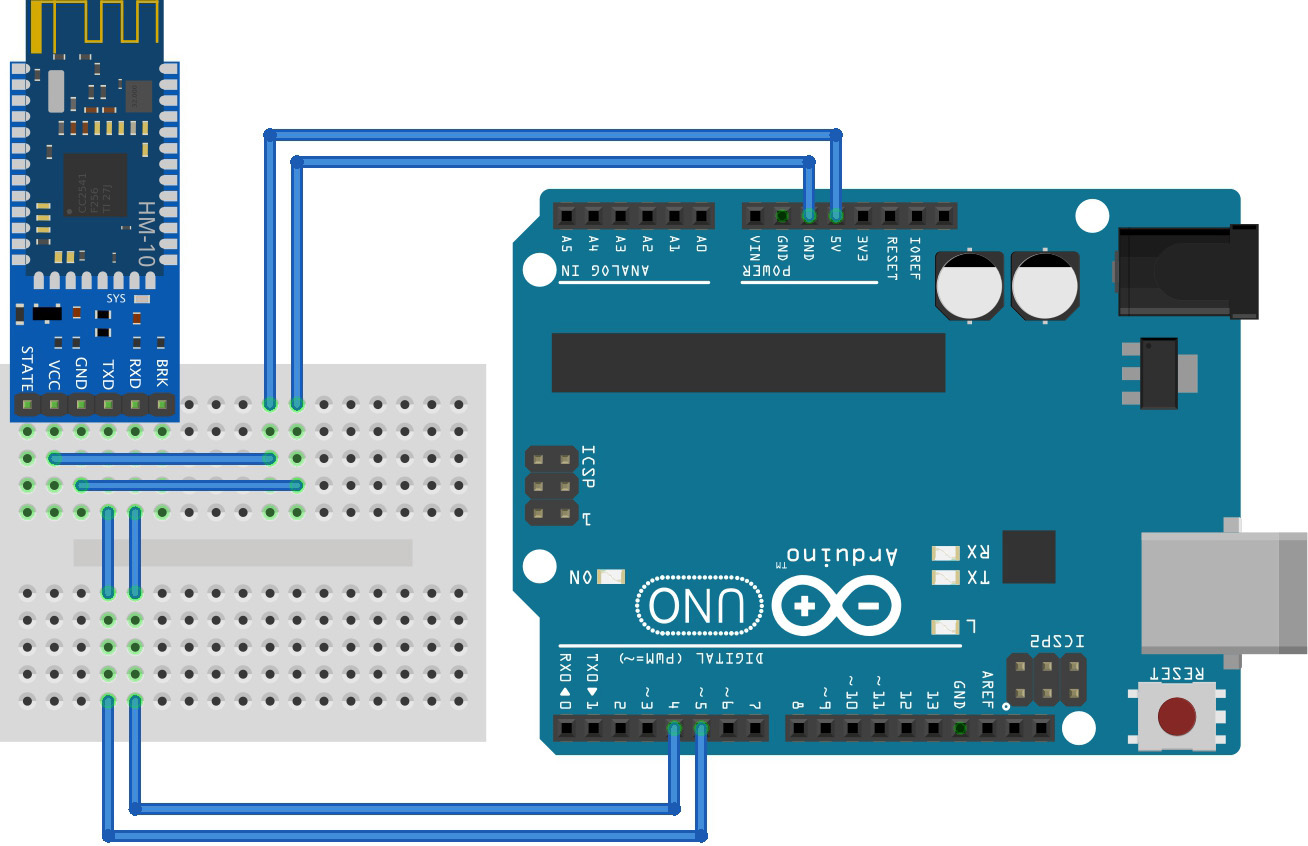
\includegraphics[width=10cm, center]{images/arduino-hm10}
\caption{Módulo Bluetooth HM10.}
\label{Rotulo}
\end{figure}

Após conectar o arduino ao computador, foi utilizado sua \textit{IDE} para escrever o código, que está no apêndice A. No código do Arduino, foi estabelecido uma comunicação serial com o módulo HM-10 para enviar os comandos AT necessários. Esses comandos são para otimizar o uso da bateria e ativar a função \textit{Beacon} do módulo. A seguir, a descrição dos comandos.

\begin{tabular}{|c|c|}
\hline 
Código & Descrição \\ 
\hline 
AT+RENEW & Coloca nos padrões de fábrica \\ 
\hline 
AT+RESET & Reinicia para aplicar os padrões de fábrica \\ 
\hline 
AT+MARJ0xNNNN & Define o valor Marjor \\ 
\hline 
AT+MINO0xNNNN & Define o valor Minor \\ 
\hline 
AT+NAMEMeuBeacon & Define o nome do dispositivo \\ 
\hline 
AT+ADVI5 & Define tempo de envio. 5 = 546.25 millisegundos \\ 
\hline 
AT+ADTY3 & Define como não pareável \\ 
\hline 
AT+IBEA1 & Habilita como Beacon \\ 
\hline 
AT+DELO2 & Configura para apenas emitir sinal \\ 
\hline 
AT+PWRM0 & Habilita função auto-sleep para economizar energia \\ 
\hline 
AT+RESET & Reinicia para aplicar as configurações \\ 
\hline 
\end{tabular} 

Após configurado, pode ser ligado em uma bateria 3v para utilização.

\subsection{Referências}

\href{ftp://imall.iteadstudio.com/Modules/IM130614001_Serial_Port_BLE_Module_Master_Slave_HM-10/DS_IM130614001_Serial_Port_BLE_Module_Master_Slave_HM-10.pdf}{HM-10 Bluetooth 4.0 BLE module Datasheet}
\\
\href{https://www.arduino.cc/en/main/software}{Arduino IDE}
\\
\href{https://github.com/metractive/beacon-study}{Repositório da Metractive - Como construir Beacons}

\section{Módulo do Ônibus}

\subsection{Hardware}

\begin{itemize}
\item Intel Edison
\item Raspberry Pi 3
\item Tela LCD 7" (em breve)
\item NEO u-blox 6 GPS Modules
\end{itemize}

\subsubsection{Intel Edison}

\begin{figure}[!h]
\centering
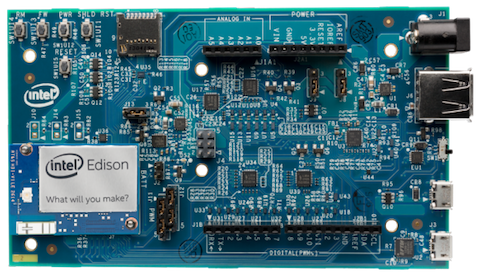
\includegraphics[width=10cm, center]{images/intel-edison-arduino-kit}
\caption{Intel Edison.}
\label{Rotulo}
\end{figure}

Inicialmente foi adotado o Intel Edison com placa de expansão arduino. Foi escolhido devido a fácil acesso a um exemplar e ótimo hardware. Ele conta com WiFi, Bluetooth, portas I/O, processador Intel Atom de 500 MHz, 1GB de memória RAM DDR3 e 4GB eMMC. \\
Sua utilização foi fácil e não obtivemos nenhuma dificuldade em instalar o sistema que escolhemos.


Problemas encontrados em adotar como solução:
\\

\textbf{Preço}

Embora tenha um ótimo hardware e uma empresa séria por trás da sua construção, o preço, em 07/2017, que gira em torno de R\$ 600,00, não justifica sua adoção como a melhor solução para o projeto já que existem alternativas com preços melhores e bom desempenho.
\\

\textbf{Ausência de controlador gráfico}

Uma das features do projeto é emitir alertas visuais para o motorista por meio de telas LCDs. A placa Intel Edison nos permite fazer alertas visuais utilizando LEDs e afins. 
\\

\textbf{Descontinuidade da placa pela Intel}

em 07/2017, a Intel anunciou a descontinuidade do desenvolvimento de algumas placas que fabrica. O Intel Edison foi uma delas.

\subsubsection{Raspberry Pi 3}

Testes realizados no Raspberry Pi 3 demonstraram ser uma boa alternativa ao Intel Edison. Foi fácil a instalação do sistema e a placa vem com saída HDMI permitindo utilizar telas LCD para fazer os alertas visuais.
Seu preço, em 08/2017, gira em torno de R\$ 150,00, 1/4 do preço do Intel Edison. Seu hardware contém boas especificações.

Embora tenha um hardware com especificações superiores ao Intel Edison, não houve ganho de desempenho ao rodar o sistema, devido a ausência de algoritmos complexos no sistema. Assim, a grande vantagem de se utilizar o Raspberry Pi 3 ao invés do Intel Edison, é seu baixo custo e recurso de chip gráfico.

\subsubsection{Módulo NEO u-blox 6 GPS}



Para realizar o rastreamento do ônibus foi adotado o módulo NEO u-blox 6 GPS Modules, devido a compatibilidade com as placas que contém o sistema embarcado e preço acessível. 




\subsection{Software}

\subsubsection{Sistema Operacional}

\textbf{Android Things}
Em 2016 o Google anunciou o Android Things, uma versão do Android voltada para IoT (Internet of Things). Ele é, atualmente, uma versão do Android Marshmallow reduzida. Sua escolha foi devido a facilidade de embarcar em placas como o Raspberry Pi e Intel Edison, e a variedade de recursos que já estão disponíveis no SO que facilitam o desenvolvimento do módulo, como o recurso LocationManager. \textbf{[Detalhar mais essa parte]}

\subsubsection{IDE}

Foi escolhido o Android Studio como IDE do projeto. Ela é desenvolvida pela IntelliJ e tida pelo Google como ferramenta oficial de desenvolvimento para aplicativos Android.

\subsubsection{Linguagem}

O Google tem duas linguagens de primeiro nível para desenvolvimento Android: Java e Kotlin. Para esse projeto adotamos a linguagem Kotlin, que possui sintaxe muito simplificado em comparação ao Java. Embora Java tenha sido a primeira linguagem oficial para desenvolvimento, Kotlin oferece acesso aos mesmo recursos do sistema.
Algumas bibliotecas disponíveis, desenvolvidas por terceiros, ainda não migraram para o Kotlin, obrigando a implementar algumas classes em Java. Como Kotlin tem interoperabilidade com Java, não existe nenhum impeditivo de utilizar Kotlin e eventualmente alguma classa Java.

\subsubsection{Arquitetura}

\begin{figure}[!h]
\centering
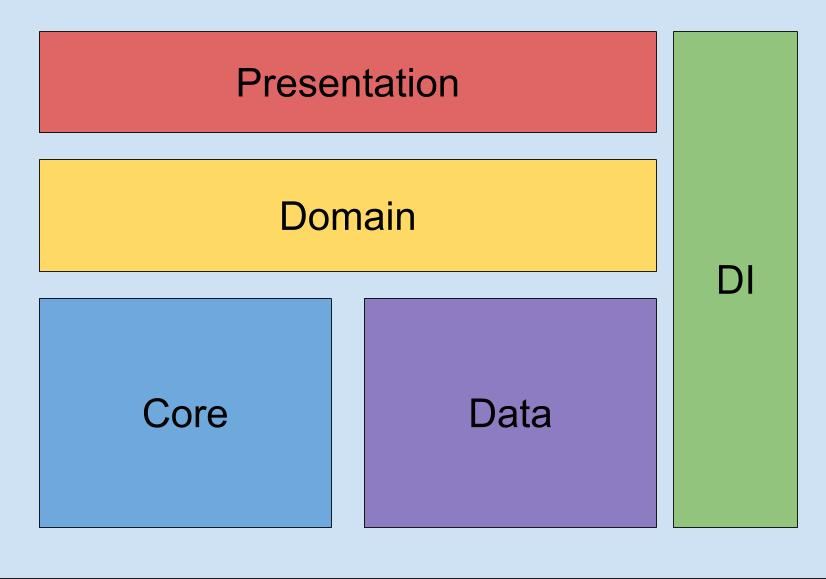
\includegraphics[width=10cm, center]{images/brick_diagram_bus_tracker}
\caption{Diagrama de bloco do módulo do ônibus.}
\label{Rotulo}
\end{figure}

Para desenvolvimento do software, foi adotado o padrão \textit{Clean Archtecture}. É um padrão que visa um maior desacoplamento das classes e distruibui bem as responsabilidades.

\begin{description}

\item[Core] Não contém nenhuma lógica de negócio. Esta camada provê informações comuns, como configurações estáticas da placa a toda a aplicação. Possui também algumas classes e interfaces bases.

\item[Data] Responsável por prover dados para toda aplicação. Ela adota o Padrão de Arquitetura \textit{Repository}, tendo uma interface de acesso aos dados. Uma grande vantagem em utilizar essa camada com esse padrão de arquitetura, é o respeito a responsabilidade única, um dos princípios do \textit{SOLID}. Ela encapsula toda lógica de busca de dados, assim, caso uma classe precise de algum dado específico, ela solicita através da interface de comunicação e a classe que implementa a interface, cuida de toda lógica de busca de dado, seja um dado armazenado localmente, em cache ou em um servidor remoto. Tudo fica transparente para a classe que solicitou o dado.

\item[Domain] Esta camada encapsula toda regra de negócios da aplicação. Toda vez que é necessário realizar processamentos em dados para satisfazer funcionalidades, é feito por esta camada.

\item[Presentation] Responsável por toda interface gráfica. Toda lógica de criação de telas e interceptação de interações do usuário com o aplicativo, é feito aqui. Quando é necessário procurar dados para exibir ao usuário, é feito solicitações deles para a camada Domain ou Data para que seja possa exibir os dados.
 
\end{description}

\subsubsection{Animações}

Um dos tópicos mais presentes sobre melhorar experiência do usuário em sistemas, são as animações. Elas deixam o uso mais fluído e agradável para o usuário. [pesquisar na literatura e colocar aqui]\\

O \textit{Android Things} provê uma \textit{API} para animações que herdou da versão do \textit{Android} de smartphones. Ela foi utilizada para melhorar a experiência de uso dos motoristas com o módulo, porém, foi observado uma baixa qualidade nas animações. O que fez ter o efeito contrário, pois passa a impressão de ser um sistema de baixo desempenho.\\

[PESQUISAR MELHOR SOBRE QUALIDADES ALCANÇADAS DE FPS)

\subsubsection{Referências}

%links do intel edison
\href{https://software.intel.com/en-us/iot/hardware/edison}{Site Oficial Intel Edison}\\
\href{http://download.intel.com/support/edison/sb/edisonmodule_hg_331189004.pdf}{Datasheet Intel Edison}\\
\href{https://www.embarcados.com.br/placas-intel-edison-galileo-e-joule-serao-descontinuadas/}{Anúncio do fim da produção do Intel Edison}\\
%links do raspberry pi
\href{https://www.raspberrypi.org/products/raspberry-pi-3-model-b/}{Site Oficial Raspberry Pi}\\
\href{https://www.raspberrypi.org/documentation/hardware/computemodule/RPI-CM-DATASHEET-V1_0.pdf}{Datasheet Raspberry Pi 3}\\
%links do módulo GPS
\href{https://www.u-blox.com/sites/default/files/products/documents/NEO-6_DataSheet_(GPS.G6-HW-09005).pdf}{Datasheet NEO u-blox 6 GPS Modules}\\
%android things
\href{https://developer.android.com/things/index.html}{Site Oficial Android Things}\\
\href{https://developer.android.com/things/hardware/edison.html}{Configuração do Android Things no Intel Edison}\\
\href{https://developer.android.com/things/hardware/raspberrypi.html}{Configuração do Android Things no Raspberry Pi 3}\\

\newpage

\section{Aplicativo}

\subsection{Telas}

\begin{figure}[h]
\centering
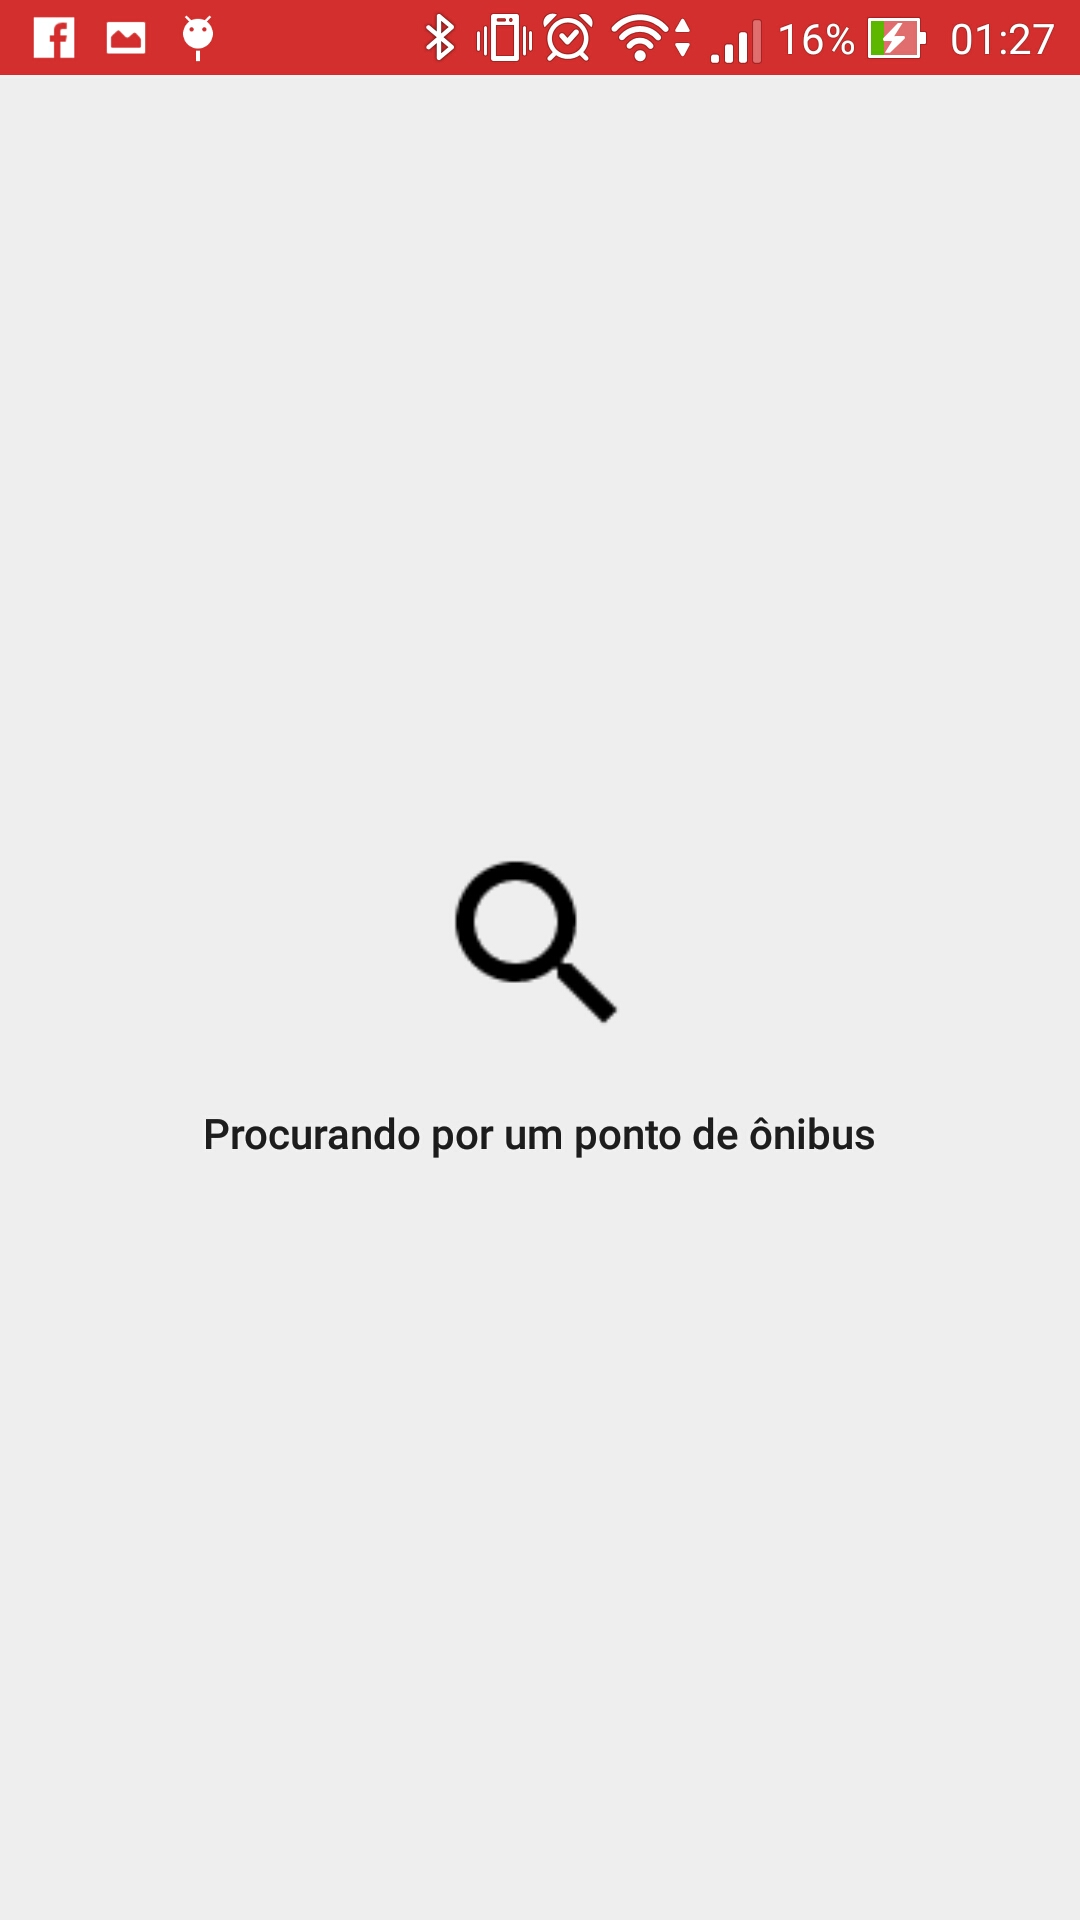
\includegraphics[width=5cm, center]{images/beacon_searching_bus_stop}
\caption{Tela de busca por um ponto de ônibus do aplicativo móvel.}
\label{Rotulo}
\end{figure}

\begin{figure}[h]
\centering
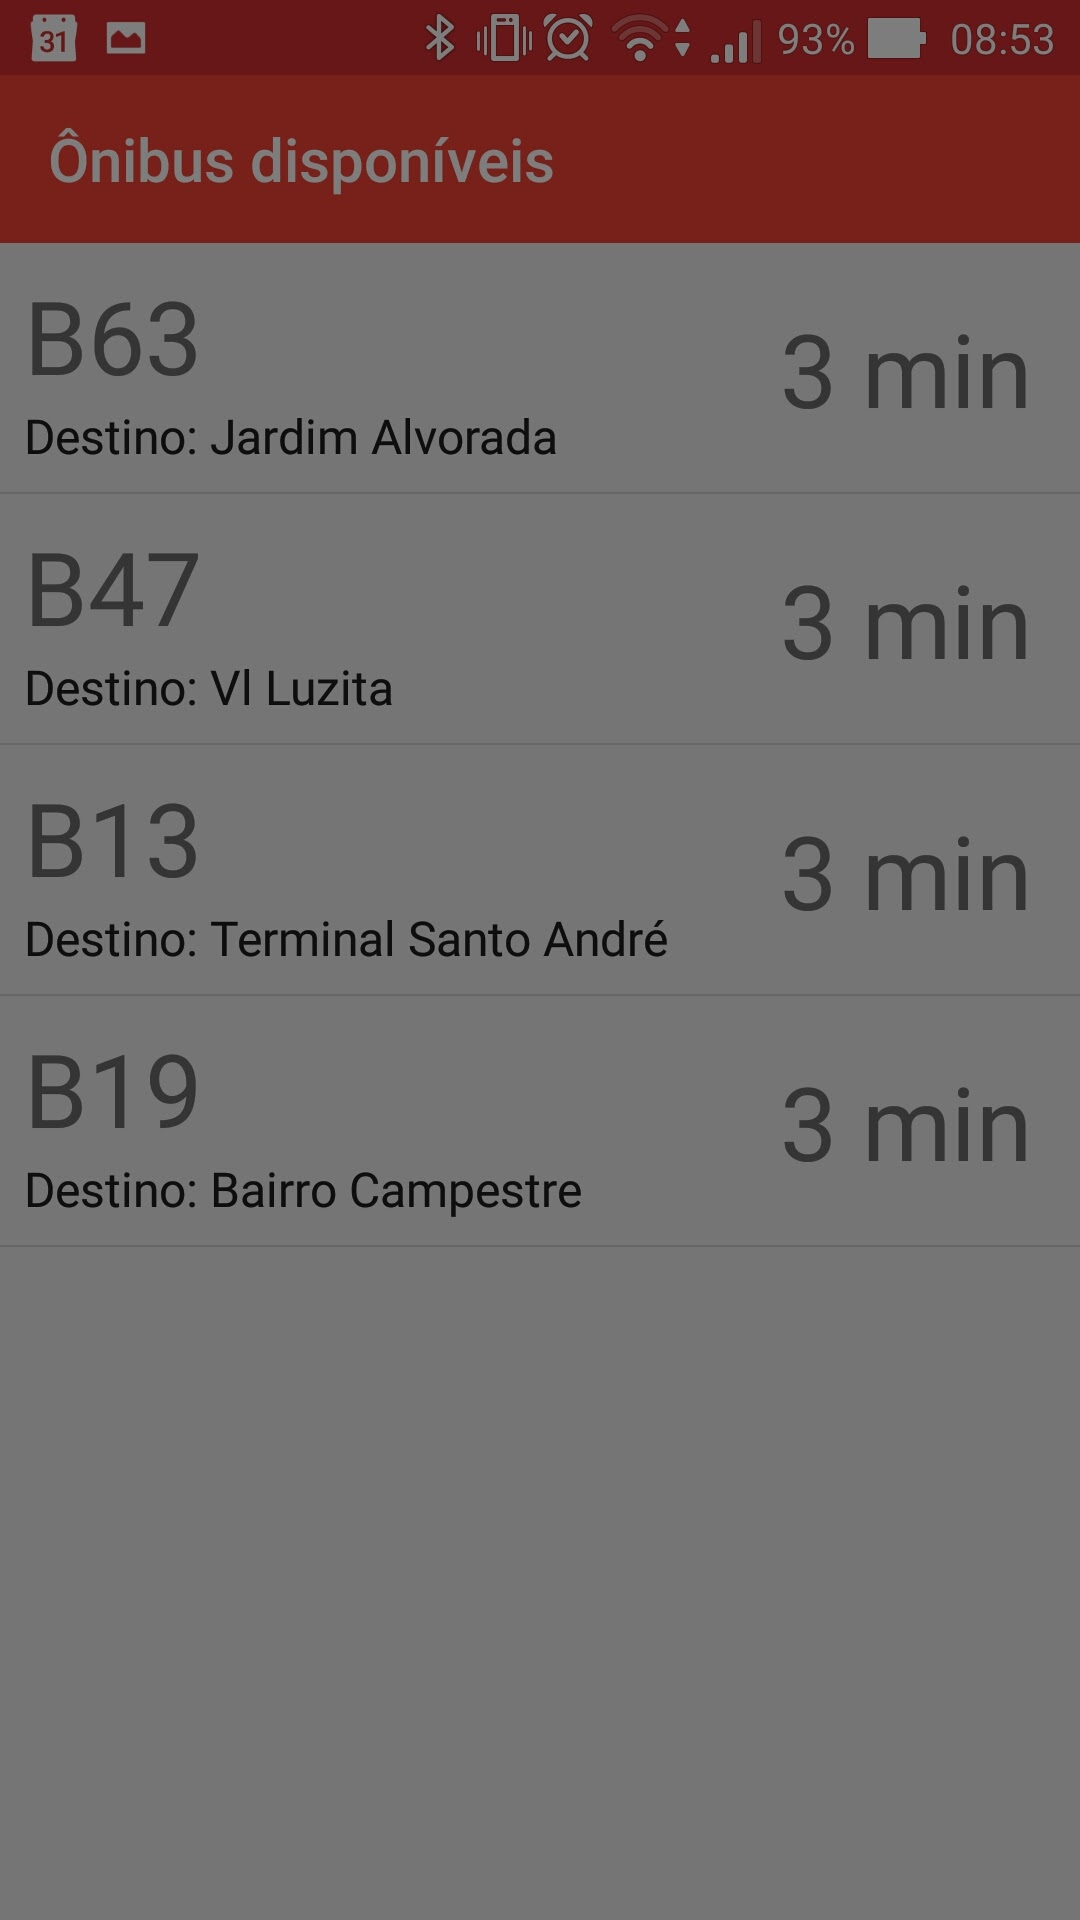
\includegraphics[width=5cm, center]{images/beacon_list_bus}
\caption{Tela com lista de ônibus disponíveis do aplicativo móvel.}
\label{Rotulo}
\end{figure}

\begin{figure}[h]
\centering
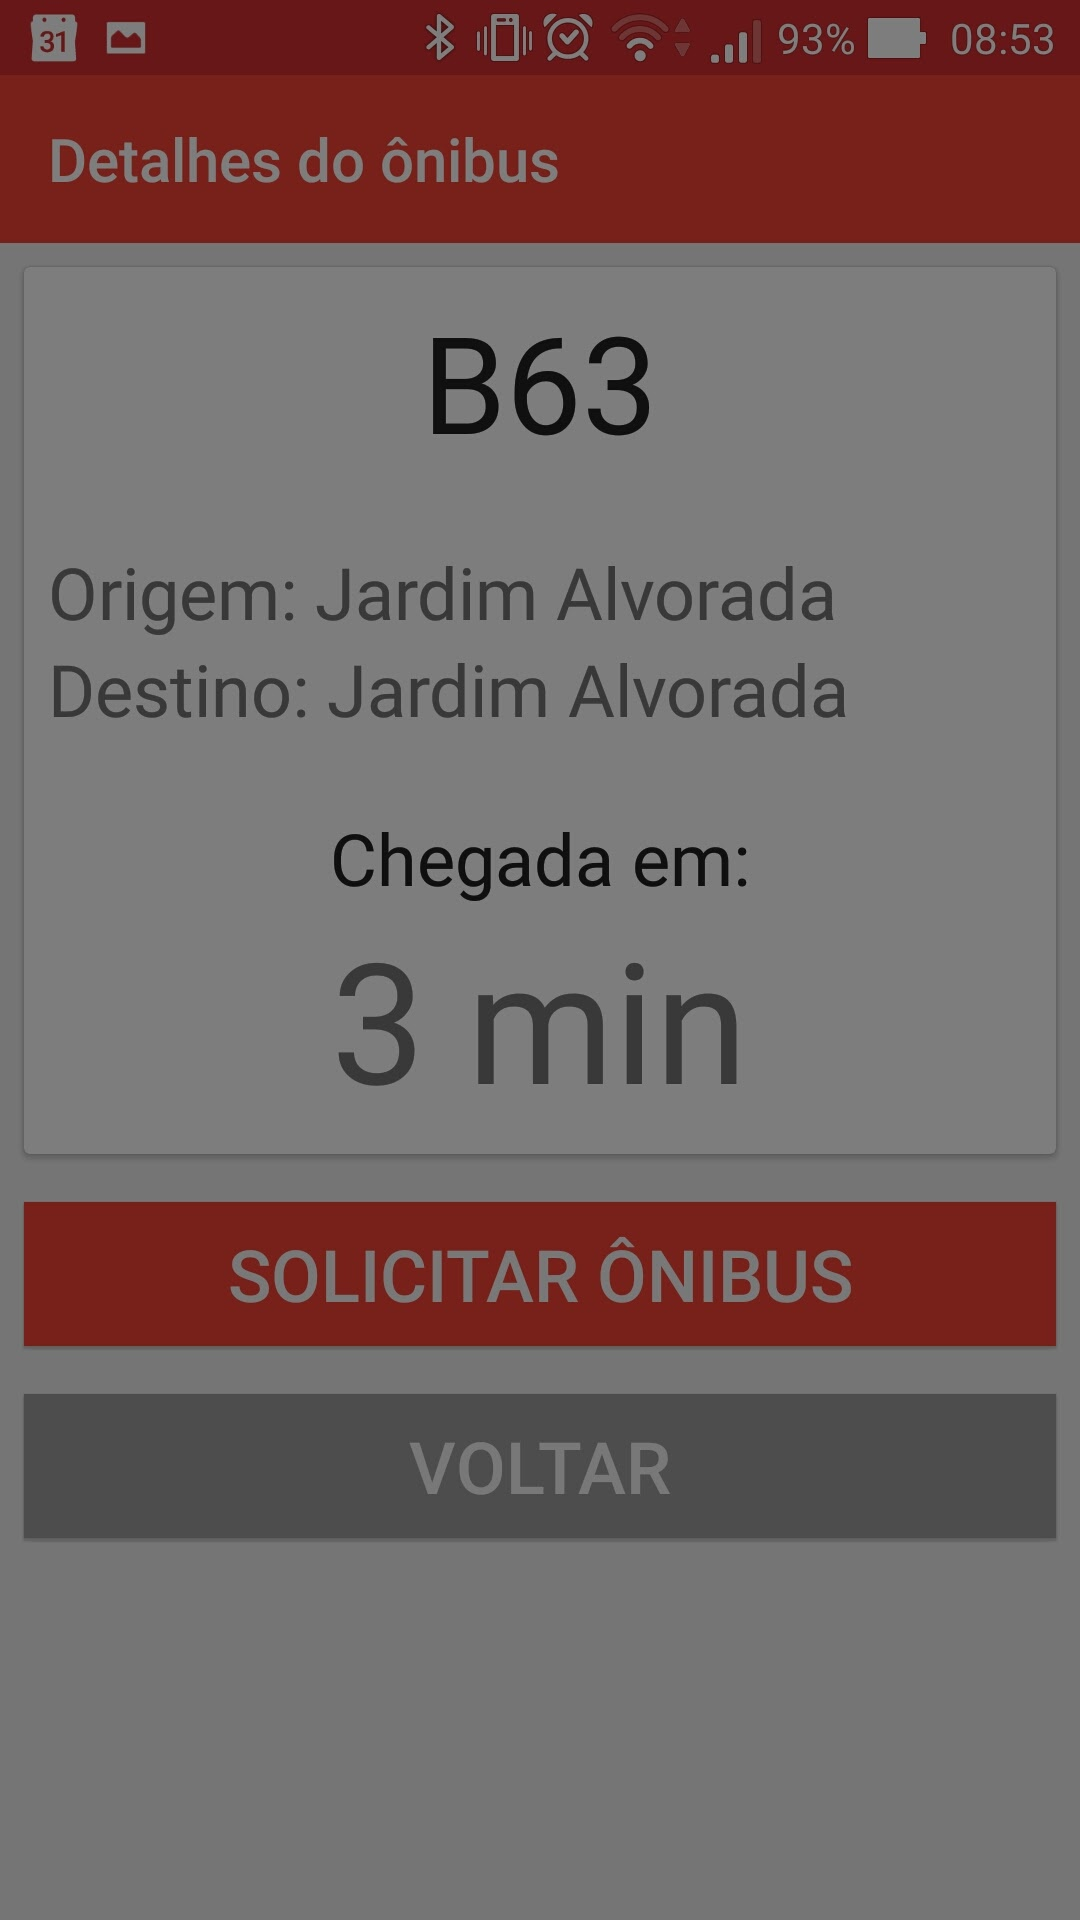
\includegraphics[width=5cm, center]{images/beacon_detail_bus}
\caption{Tela com detalhes do ônibus do aplicativo móvel.}
\label{Rotulo}
\end{figure}

\newpage

\subsection{IDE}

Foi escolhido o Android Studio como IDE do projeto. Ela é desenvolvida pela IntelliJ e tida pelo Google como ferramenta oficial de desenvolvimento para aplicativos Android.

\subsection{Linguagem}

O Google tem duas linguagens de primeiro nível para desenvolvimento Android: Java e Kotlin. Para esse projeto adotamos a linguagem Kotlin, que possui sintaxe muito simplificado em comparação ao Java. Embora Java tenha sido a primeira linguagem oficial para desenvolvimento, Kotlin oferece acesso aos mesmo recursos do sistema.
Algumas bibliotecas disponíveis, desenvolvidas por terceiros, ainda não migraram para o Kotlin, obrigando a implementar algumas classes em Java. Como Kotlin tem interoperabilidade com Java, não existe nenhum impeditivo de utilizar Kotlin e eventualmente alguma classa Java.

\newpage

\subsection{Arquitetura}

\begin{figure}[h]
\centering
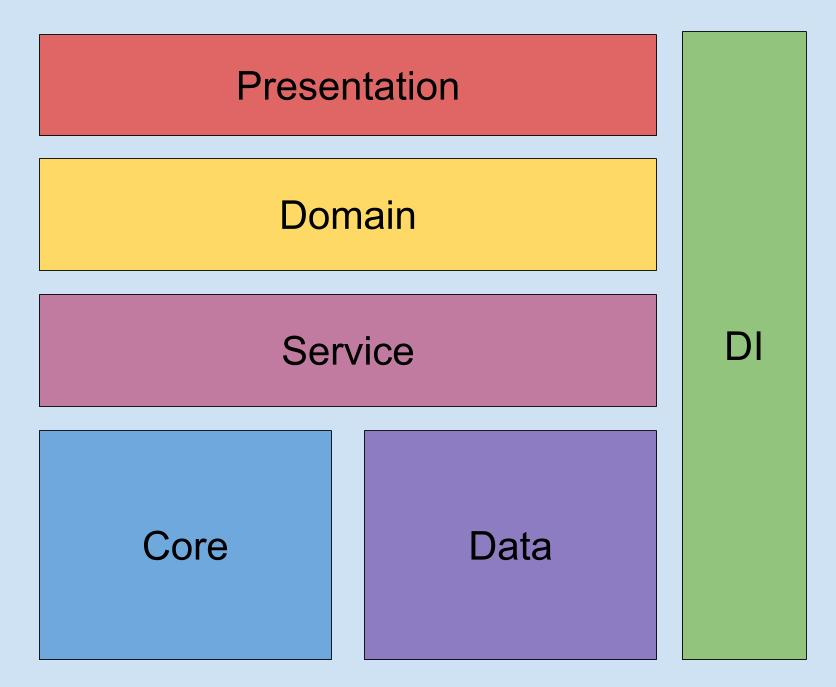
\includegraphics[width=10cm, center]{images/brick_diagram_beacon}
\caption{Diagrama de blocos do aplicativo móvel.}
\label{Rotulo}
\end{figure}

Para desenvolvimento do software, foi adotado o padrão \textit{Clean Architecture}. É um padrão que visa um maior desacoplamento das classes e distruibui bem as responsabilidades.

\begin{description}

\item[Core] Não contém nenhuma lógica de negócio. Esta camada provê informações comuns, como configurações estáticas da placa a toda a aplicação. Possui também algumas classes e interfaces bases.

\item[Data] Responsável por prover dados para toda aplicação. Ela adota o Padrão de Arquitetura \textit{Repository}, tendo uma interface de acesso aos dados. Uma grande vantagem em utilizar essa camada com esse padrão de arquitetura, é o respeito a responsabilidade única, um dos princípios do \textit{SOLID}. Ela encapsula toda lógica de busca de dados, assim, caso uma classe precise de algum dado específico, ela solicita através da interface de comunicação e a classe que implementa a interface, cuida de toda lógica de busca de dado, seja um dado armazenado localmente, em cache ou em um servidor remoto. Tudo fica transparente para a classe que solicitou o dado.

\item[Service] Provê serviços para qualquer camada. No caso do aplicativo, a implementação do serviço de voz fica neste pacote e é injeta pelo pacote de Injeção de Dependências.

\item[Domain] Esta camada encapsula toda regra de negócios da aplicação. Toda vez que é necessário realizar processamentos em dados para satisfazer funcionalidades, é feito por esta camada.

\item[Presentation] Responsável por toda interface gráfica. Toda lógica de criação de telas e interceptação de interações do usuário com o aplicativo, é feito aqui. Quando é necessário procurar dados para exibir ao usuário, é feito solicitações deles para a camada Domain ou Data para que seja possa exibir os dados.

\item[DI] Este projeto utiliza o padrão de arquitetura \textit{Injeção de Dependências}. Esta camada provê todas dependências, fazendo a implementação mais limpas nas outras classes, já que não precisam saber como instânciar uma classe, apenas usam.
 
\end{description}

\subsection{Áudio Descrição}

Uma das funcionalidades do aplicativo é descrição da tela que o deficiente está. O \textit{TalkBack} fala para o usuário em qual componente ele está tocando, porém, não descreve em qual tela ele acabou de entrar. 
A implementação por áudio descrição foi simples com uso da API nativa \textit{TextToSpeech}, onde podemos passar textos personalizados e o serviço se encarrega de sintetizar a voz.

O uso de uma camada de DI (Injeção de Dependências) facilitou o processo de implementação, fazendo ela na camada de serviço e configurando a instanciação no padrão \textit{Singleton} para que todos que vão utilizar (nesse caso são os \textit{presenters}), apenas solicitem a instância sendo passada por construtor.

\subsection{Usabilidade}

É uma boa prática no desenvolvimento de softwares, sempre confirmar se o usuário tem certeza que deseja executar alguma alteração que possa ter algum impacto no sistema ou em alguma funcionalidade, normalmente lançando alertas para garantir que o usuário não clicou sem querer em algum determinado botão, por exemplo. 

Inicialmente foi pensado em usar um \textit{dialog} para que o usuário confirme a ação de adicionar um ônibus como favorito, na tela de confirmação de acompanhamento. Ao testar a aplicação funcionando com \textit{Talkback}, foi observado que o sistema descreve o botão com o seguinte texto: \textit{"Adicionar aos favoritos. Botão, para acionar toque duas vezes"}. Esse texto já faz o usuário se assegurar da sua ação, tornando a prática de lançar um alerta ser algo desnecessário, fazendo o usuário ter um trabalho a mais de deslizar o dedo pela tela para encontrar os botões de \textit{OK} e cancelar do \textit{dialog.}

Com base nessas observações, não foi implementado \textit{dialogs} de confirmação. Deixando a responsabilidade de afirmar as ações do usuário para o \textit{Talkback} fazer. Embora seja uma pequena ação, tem grande impacto na usabilidade do aplicativo por parte do usuário final, que são os deficientes visuais.

O sistema operacional Android permite que aplicativos implementem variações da tela de acordo com a orientação do dispositivo, retrato ou paisagem. Isso permite que o layout do aplicativo se adapte a nova disposição de espaço.

Pensando no usuário final, para saber onde está cada elemento, ele precisa deslizar o dedo pela tela para conhecer a localização de cada um. Se ao rotacionar o aparelho, a disposição dos elementos mudar, o usuário precisa verificar novamente onde está cada um.

Como este trabalho desenvolve um aplicativo com poucos elementos na tela para simplificar o uso por deficientes visuais, foi bloqueado a mudança de tela ao rotacionar o aparelho. Isso garante um melhor conforto ao usar o aplicativo.


\section{Web service}

\subsection{Localização do ônibus}

Ter conhecimento da posição do ônibus se faz necessário para realizar a previsão de chegada em um ponto de parada. Neste trabalho, sempre que o \textit{Web Service} recebe as coordenadas geográficas do ônibus, elas são corrigidas para um ponto válido da rota que este está fazendo.

Quando o \textit{Web Service} recupera as informações da rota do veículo, ele obtém todos os pontos referentes a ela, onde cada um tem informações de latitude, longitude e se este é um ponto de parada. Então é verificado qual ponto está mais próximo a localização recebida, o mais próximo é associado ao ônibus.

O cálculo de distância é feito a partir da seguinte fórmula:

FORMULA AQUI

Para otimizar a busca pelo ponto mais apto, é feito uma busca binária, que tem complexidade \textit{O(log n)}, o que reduz o tempo de busca caso fosse usar a busca sequencial, que possui complexidade \textit{O(n)}. 

\subsubsection{Busca Binária}

\textit{"Binary search is to algorithms
what a wheel is to mechanics:
It is simple, elegant, and immensely important."}
— Udi Manber, Introduction to Algorithms


Primeiro é calculado a distância entre a localização recebida do ônibus e o primeiro ponto da rota. 
Em seguida, calculamos a distância entre a localização recebida e o ultimo ponto da rota. Com isso temos a distânciaInicio e distânciaFim. 

\begin{figure}[!h]
\centering
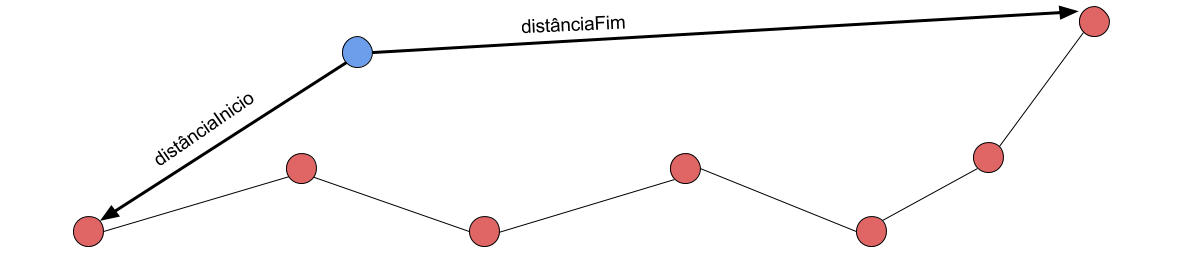
\includegraphics[width=10cm, center]{images/distanciainicio-distanciafim.png}
\caption{Representação da busca binária.}
\label{Rotulo}
\end{figure}

Um terceiro cálculo é feito, a distância entre a localização recebida e o ponto do meio da rota.

\begin{figure}[!h]
\centering
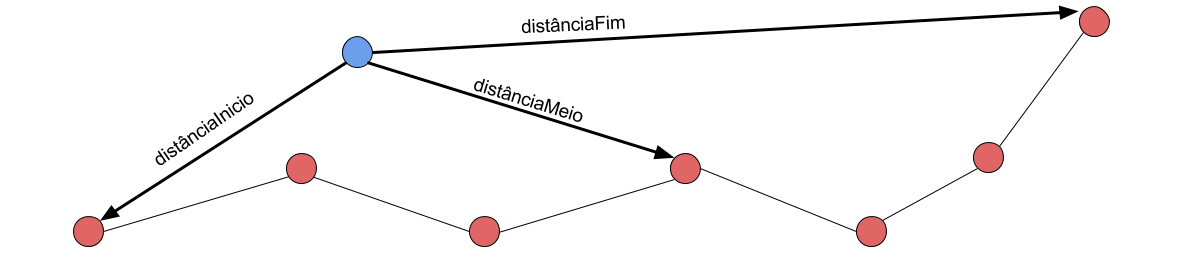
\includegraphics[width=10cm, center]{images/distanciainicio-distanciafim-distanciomeio.png}
\caption{Representação da busca binária.}
\label{Rotulo}
\end{figure}

O algoritmo então verifica qual metade é mais apta, baseando-se nas distâncias mais curtas. Se distânciaFim é maior que distânciaInicio, é feito uma recursividade assumindo distânciaMeio como fim.

\begin{figure}[!h]
\centering
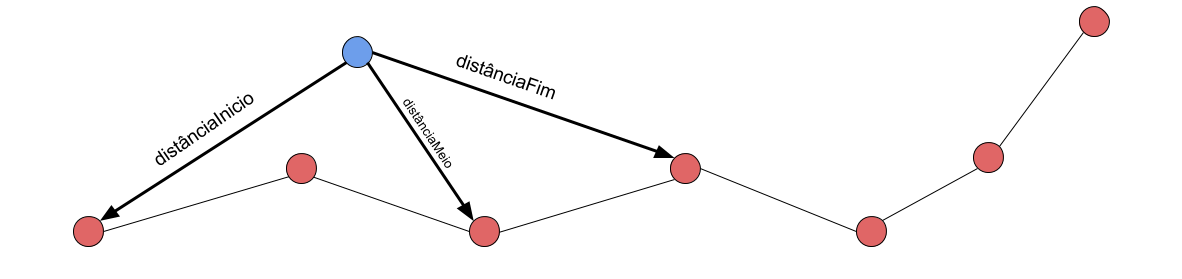
\includegraphics[width=10cm, center]{images/nova-distancia.png}
\caption{Representação da busca binária.}
\label{Rotulo}
\end{figure}

Fazendo isso sucessivamente, chega uma hora que não é mais possível dividir, então o ponto mais próximo assume o posto de mais apto e é associado ao ônibus.

\subsection{Previsão de chegada}

Para calcular a previsão de chegada de um ônibus, precisamos saber a ultima localização conhecida dele e o ponto de parada escolhido. Com essas duas informações podemos recuperar todos dados necessários para o cálculo.

Primeiro é recuperado todos os dados da rota que o ônibus está fazendo. Cada rota possui N pontos associados a ela, onde cada um tem a informação de latitude e longitude, e se este é um ponto de parada. Sabendo em qual ponto da rota o ônibus está e qual ponto de parada o usuário se encontra, podemos pegar todos os pontos que estão entre eles e calcular a distância. 

A partir dela somamos a distância dentre todos esses pontos, com isso dividimos pela velocidade da pista e sabemos quanto tempo aproximado falta para o ônibus chegar na parada.

FORMULA T = S/V


\subsection{Alertar motorista sobre parar}

O \textit{Android Things} não suporta serviço de \textit{push notification}. Para enviar mensagens instantâneas ao módulo foi utilizado o \textit{Realtime Database}, do \textit{Firebase}, que permite observar um nó. Sempre que existe uma alteração deste, quem está observando é notificado.

IMAGEM DO FIREBASE AQUI

Quando um módulo do ônibus é conectado a internet, ele cria um nó com seu ID na base de dados e um nó filho intitulado \textit{needsstop}, e passa a observá-lo. Quando o valor do nó filho é alterado, o módulo então dispara uma notificação para o motorista sobre a necessidade de parar no próximo ponto de ônibus.

O responsável por alterar o valor do nó filho é o \textit{Web Service}. Como visto na seção \textit{Localização do Ônibus}, é feito uma varredura para descobrir o ponto da rota que o ônibus se encontra. Em seguida também é verificado qual o próximo ponto que ele vai passar. Caso o próximo ponto esteja na lista de requisições de parada, é então alterado o valor do nó filho para que aquele módulo alerte o motorista.

\subsection{Alertar usuário que ônibus chegou}

Quando o motorista chega na parada, ele pressiona um botão para anunciar sua chegada. Quando \textit{Web Service} recebe esse alerta por meio de uma requisição \textit{HTTP}, ele verifica quais usuários estão aguardando aquele ônibus, então é disparado uma \textit{push notification}, por meio do \textit{Firebase}, avisando que o ônibus que ele aguarda está parado.

\subsection{Dificuldades}

Apesar de conter conceitos simples de aprender, devido à grande quantidade de métodos para se realizar os mesmos processos, fica um pouco difícil para assimilar quais os arquivos que devem ser modificados para o funcionamento adequado da aplicação.
Primeira dificuldade surgiu ao utilizar o mongoose, uma solução baseada em \textit{schemas} para o banco de dados MongoDB que cuida de validações e tipagem de dados, resolvido ao criar arquivos separados para cada \textit{collection} do banco.

\end{document}
